% !TEX program = pdflatex
% ============================================================
%  HabitIA --- TFM 2025-2026 (Universidad Complutense de Madrid)
%  Memoria y catorce anexos. Los recursos están en figuras/.
%  Compilación desde esta carpeta:
%    tectonic HabitIA_memoria.tex
%  Alternativa: pdflatex HabitIA_memoria.tex (dos pasadas).
% ============================================================
\documentclass[11pt,a4paper]{article}

% ---- Codificación y tipografía clásica de LaTeX (Latin Modern) ----
\usepackage{iftex}
\ifPDFTeX\usepackage[utf8]{inputenc}\fi
\usepackage[T1]{fontenc}
\usepackage{lmodern}
\usepackage{textcomp}

\usepackage[spanish,es-tabla,es-nodecimaldot,shorthands=off]{babel}
\usepackage[a4paper,top=2.6cm,bottom=2.3cm,left=2.5cm,right=2.5cm]{geometry}

% ---- Separación de párrafos: espacio en blanco en vez de sangrado ----
\setlength{\parindent}{0pt}
\setlength{\parskip}{0.8em}

% ---- Símbolos Unicode del texto original (€, ×, −, ≈, ≤, ≥, ², →) ----
\usepackage{newunicodechar}
\newunicodechar{€}{\texteuro}
\newunicodechar{×}{\ensuremath{\times}}
\newunicodechar{±}{\ensuremath{\pm}}
\newunicodechar{−}{\ensuremath{-}}
\newunicodechar{≈}{\ensuremath{\approx}}
\newunicodechar{≤}{\ensuremath{\le}}
\newunicodechar{≥}{\ensuremath{\ge}}
\newunicodechar{²}{\textsuperscript{2}}
\newunicodechar{→}{\ensuremath{\rightarrow}}

\usepackage{amsmath}
\usepackage{array}
\usepackage{booktabs}
\usepackage{tabularx}
\usepackage{ragged2e}
\usepackage{multirow}
\usepackage{xcolor}
\usepackage{caption}
\usepackage{enumitem}
\usepackage{needspace}
\usepackage{listings}
\usepackage{graphicx}
\graphicspath{{figuras/}}
\usepackage{tikz}
\usetikzlibrary{arrows.meta,positioning,babel}
\usepackage{pgfplots}
\pgfplotsset{compat=1.17}
\usepackage{fancyhdr}
\usepackage{titlesec}
\usepackage{xurl}
\usepackage[hidelinks,bookmarksnumbered]{hyperref}
\hypersetup{pdftitle={HabitIA: memoria y anexos},pdfauthor={Equipo HabitIA}}
\setlength{\emergencystretch}{2em}

% ---- Encabezado y pie ----
\pagestyle{fancy}
\fancyhf{}
\fancyhead[C]{\footnotesize UNIVERSIDAD COMPLUTENSE DE MADRID \textperiodcentered{} TFM 2025--2026}
\fancyfoot[C]{\footnotesize HabitIA \textperiodcentered{} \thepage}
\renewcommand{\headrulewidth}{0.4pt}
\renewcommand{\footrulewidth}{0pt}

% ---- Estilo de secciones (sans-serif) ----
\titleformat{\section}{\Large\sffamily\bfseries}{\thesection}{0.6em}{}
\titleformat{\subsection}{\large\sffamily\bfseries}{\thesubsection}{0.5em}{}
\renewcommand{\thesection}{\arabic{section}}
\renewcommand{\thesubsection}{\thesection.\arabic{subsection}}
\setcounter{secnumdepth}{2}

% ---- Tablas / captions ----
\captionsetup{font=small,labelfont=bf,labelsep=period}
\renewcommand{\tablename}{Tabla}
\renewcommand{\figurename}{Figura}
\renewcommand{\arraystretch}{1.25}
\newcolumntype{L}{>{\RaggedRight\arraybackslash}X}
\newcommand{\fuente}[1]{\par\vspace{2pt}{\footnotesize\itshape #1}\par}
\newcommand{\thead}[1]{\textbf{#1}}

% ---- Leyenda de diagramas en anexos ----
\newcommand{\figcap}[1]{\par\vspace{3pt}{\footnotesize\textbf{#1}}\par\vspace{4pt}}

% ---- Código ----
\definecolor{codebg}{gray}{0.96}
\lstset{
  basicstyle=\ttfamily\footnotesize,
  breaklines=true,columns=fullflexible,keepspaces=true,
  showstringspaces=false,frame=single,rulecolor=\color{gray!45},
  backgroundcolor=\color{codebg},xleftmargin=8pt,framexleftmargin=8pt,
  aboveskip=8pt,belowskip=8pt
}

% ---- Anexos (numeración propia 1..14, fuera del índice principal) ----
% Cada anexo y sub-anexo se escribe en el cuerpo como \section*{...} /
% \subsection*{...} literales (no como una macro envolvente), a propósito:
% el panel de estructura/outline de VSCode y de LaTeX Workshop escanea el
% código fuente en busca de \section, \subsection, etc. de forma literal y
% NO expande macros, así que envolverlos en un \newcommand los dejaría
% invisibles para ese panel aunque el PDF se viera idéntico. Al ser
% \section*/\subsection* con asterisco no se numeran automáticamente (el
% número "1", "1 1"... se escribe a mano con \theanexo) ni se añaden al
% \tableofcontents principal, que conserva solo la lista de la memoria.
\newcounter{anexo}
\newcounter{anexosub}[anexo]

\begin{document}
\hypersetup{pageanchor=false}

% ============================= PORTADA (MEMORIA) =============================
\begin{titlepage}
\thispagestyle{empty}
\centering
\vspace*{0.6cm}
{\Large UNIVERSIDAD COMPLUTENSE DE MADRID\par}
{\Large FACULTAD DE ESTUDIOS ESTADÍSTICOS\par}
\vspace{1 cm}
{\Large Máster Big data, Data Science e\par}
{\Large Inteligencia Artificial 2025-2026\par}
\vspace{1.3cm}

\includegraphics[width=3.1cm]{ucm-logo.png}
\vspace{1.3cm}

{\Large \textbf{Trabajo Fin de Máster: HabitIA}\par}
\vspace{1cm}
{\large Equipo:\par}
\vspace{0.2cm}
{\large Mauricio Peón García\par}
{\large João Paulo Nogueira Cunha\par}
{\large Manuel Macedo Púlido\par}
{\large Aldo Mauricio Ress Vilet\par}
{\large Tomás Perales Lara\par}
\vspace{1 cm}
{\small Madrid \textperiodcentered{} Curso 2025--2026\par}
\end{titlepage}

% ============================= ÍNDICE =============================
\clearpage
\renewcommand{\contentsname}{Índice}
\begingroup
\setlength{\parskip}{0pt}
\thispagestyle{empty}
{
\hypersetup{linkcolor=black}
\tableofcontents
}
\endgroup

% ============================= 1 =============================
\clearpage
\pagenumbering{arabic}
\setcounter{page}{1}
\hypersetup{pageanchor=true}
\section{Resumen}

Buscar vivienda en Madrid obliga a comparar cientos de anuncios heterogéneos sin una referencia objetiva de si el precio pedido es razonable para lo que se ofrece. Este trabajo presenta HabitIA, una aplicación que combina un modelo de estimación del precio de la vivienda con un buscador y un asistente conversacional para ayudar a encontrar y comparar pisos de compra y alquiler en Madrid capital.

El desarrollo del modelo partió de 75.469 viviendas del conjunto público \emph{idealista18}, anunciadas en 2018 y enriquecidas con tres indicadores municipales de barrio: el alquiler mediano, un índice de vulnerabilidad y una tasa de incidencias de seguridad. Tras seleccionar las variables por su contribución al ajuste y comparar regresión lineal, Random Forest y XGBoost mediante validación cruzada, se eligió un XGBoost de 410 árboles y 21 variables que puede construirse con la información de un anuncio actual. En un conjunto de prueba de 15.094 viviendas reservado durante el ajuste y la comparación de modelos, su error porcentual mediano es del 9,3 \% y el 80,6 \% de las estimaciones se desvía menos de un 20 \% del precio anunciado. La superficie y la localización explican la mayor parte de sus predicciones.

Para aplicar el modelo hoy, las variables se reconstruyen a partir de la API de Idealista, incluida la extracción de equipamientos desde la descripción del anuncio, y la estimación se actualiza a 2026 con un índice de precios por distrito. Sobre 412 anuncios reales de 2026, la mediana del cociente entre precio pedido y estimación es de 1,003. La aplicación web ordena los anuncios con una puntuación que combina la relación entre precio y estimación con el entorno y el tiempo de desplazamiento, según los pesos que elige cada persona, y un asistente basado en un modelo de lenguaje permite realizar las mismas tareas conversando, obteniendo siempre las cifras de herramientas deterministas.

El trabajo tiene límites claros: el modelo aprende precios anunciados y no de cierre, su actualización a 2026 depende de proyecciones, y la renta mensual se deriva de ratios de distrito sin validación independiente. El código, los cuadernos de análisis y el modelo están publicados para su reproducción [6].

\textbf{Palabras clave:} valoración de vivienda, XGBoost, SHAP, Madrid, modelos de lenguaje, agentes con herramientas.

% ============================= 2 =============================
\section{Introducción}

\subsection{Motivación}

Quien busca vivienda en Madrid se enfrenta a una oferta amplia y dispersa, a anuncios que describen de forma desigual inmuebles muy distintos y a precios que han crecido con rapidez: según la estadística registral del Ayuntamiento, el precio medio de compraventa ha aumentado en torno a un 6 \% anual en el distrito mediano desde 2018 (capítulo~\ref{sec:produccion}). Comparar dos pisos exige tener en cuenta a la vez la superficie, la planta, el equipamiento y la ubicación, y además las circunstancias de cada persona: su presupuesto, sus requisitos imprescindibles o el tiempo que está dispuesta a dedicar a desplazarse al trabajo.

Los portales inmobiliarios permiten filtrar por características, pero no indican si un precio es alto o bajo para una vivienda concreta. Los modelos de valoración automática responden a esa pregunta, aunque suelen estar pensados para profesionales y su funcionamiento no es transparente para quien busca casa. HabitIA parte de la idea de que ambas piezas se refuerzan: una referencia de precio es más útil dentro del propio flujo de búsqueda, y la búsqueda es más útil si ayuda a interpretar cada anuncio.

Un matiz condiciona todo el trabajo. Los datos disponibles recogen precios anunciados, no precios de compraventa, de modo que la referencia que produce el modelo es el precio de oferta típico de una vivienda de esas características, no una tasación. Que un anuncio quede por debajo de la referencia es una razón para revisarlo con atención, no la prueba de que sea una ganga.

\subsection{Objetivos}

El objetivo general es desarrollar una herramienta que ayude a buscar y comparar vivienda en Madrid capital apoyándose en un modelo de estimación de precios construido y evaluado con rigor. Este objetivo se concreta en los cinco objetivos específicos de la Tabla~\ref{tab:objetivos}, cada uno de los cuales se desarrolla en un capítulo de la memoria.

\begin{table}[!htb]
\centering
\caption{Objetivos específicos del trabajo.}
\label{tab:objetivos}
\begin{tabularx}{\linewidth}{@{}l L c@{}}
\toprule
& \thead{Objetivo} & \thead{Capítulo} \\
\midrule
O1 & Construir un conjunto de datos de vivienda enriquecido con información de barrio, controlando duplicados y fugas de información & 3 \\
O2 & Seleccionar variables y modelo con un procedimiento reproducible que separe entrenamiento, validación y prueba & 4 \\
O3 & Evaluar la precisión del modelo, identificar dónde falla e interpretar qué ha aprendido & 5 \\
O4 & Aplicar el modelo a anuncios actuales y delimitar su dominio de validez & 6 \\
O5 & Integrar el modelo en una aplicación web con buscador, puntuación personalizable y asistente conversacional & 7 \\
\bottomrule
\end{tabularx}
\end{table}

\subsection{Alcance y estructura de la memoria}

La herramienta cubre el municipio de Madrid y las viviendas que el modelo puede representar: pisos, estudios, dúplex y áticos de hasta 367 m². Quedan fuera las casas y chalets, las viviendas a reformar y las ocupadas, por las razones que se exponen en el capítulo~\ref{sec:produccion}. La estimación de venta procede de un modelo evaluado; en alquiler, la aplicación ofrece una referencia derivada de la venta que se presenta como tal.

Tras esta introducción, el capítulo~3 describe los datos y su análisis exploratorio; el capítulo~4, la metodología de selección de variables y modelos; el capítulo~5, los resultados en el conjunto de prueba, la interpretación del modelo y su sensibilidad; el capítulo~6, la adaptación del modelo a anuncios actuales; el capítulo~7, la aplicación y su asistente conversacional, y el capítulo~8, las conclusiones. Los anexos recogen el detalle técnico del modelo, de las tablas territoriales, de la reproducción del análisis y de la integración.

% ============================= 3 =============================
\section{Datos}

El modelo combina un conjunto público de anuncios de vivienda, que aporta el precio y las características de cada inmueble, con varias fuentes municipales que describen su entorno. Este capítulo resume cómo se construyó el conjunto de trabajo y los hallazgos exploratorios que condicionaron el modelado; el detalle completo está en los cuadernos 00 y 01 del repositorio [6].

\subsection{Fuente principal: anuncios de Idealista de 2018}

El punto de partida es \emph{idealista18} [1], que recoge los anuncios de viviendas en venta publicados en Idealista durante 2018. Para Madrid contiene 94.815 anuncios de 75.804 inmuebles distintos, ya que una vivienda aparece una vez por cada trimestre en que estuvo a la venta. Junto a las características del anuncio (superficie, habitaciones, baños, planta y equipamiento), incluye información catastral del edificio y distancias al centro, al metro más cercano y al eje de la Castellana.

Dos rasgos de estos datos condicionan todo el trabajo. El precio es el que pide el vendedor, no el de la compraventa final, por lo que las estimaciones deben entenderse como una referencia de mercado y no como una tasación. Además, las coordenadas incorporan un desplazamiento aleatorio de anonimización de unos 45 metros de media, lo que limita la resolución espacial fiable a unos 100 metros.

\subsection{Construcción del conjunto de trabajo}

Para que una vivienda anunciada durante varios trimestres no pesara varias veces en el entrenamiento, se conservó un único registro por inmueble: el de menor precio, por ser previsiblemente el más próximo al precio de cierre. La variable objetivo es, por tanto, el precio mínimo anunciado de cada inmueble en 2018.

Como unidad geográfica se eligió el barrio (131 en Madrid) y no la sección censal. Con unas 2.440 secciones y el ruido de las coordenadas, el 91,5 \% de los anuncios quedaba a menos de 77 metros de un límite de sección, de modo que muchos podían asignarse a la sección equivocada. Cada anuncio se asignó a su barrio mediante un cruce espacial con la cartografía censal del INE [9]. En este paso se detectó que el campo \texttt{LOCATIONID} de Idealista, aunque tiene formato de código de sección censal, identifica zonas internas del portal: el cruce por ese campo coincidía en 119 de 135 códigos y parecía correcto, pero asociaba anuncios a secciones que no les correspondían.

\subsection{Variables de contexto territorial}

A las características de cada anuncio se añadieron las variables de entorno de la Tabla~\ref{tab:enriquecimiento}.

\begin{table}[!htb]
\centering
\caption{Variables de contexto incorporadas al conjunto de datos.}
\label{tab:enriquecimiento}
\begin{tabularx}{\linewidth}{@{}l L l l@{}}
\toprule
\thead{Variable} & \thead{Fuente} & \thead{Periodo} & \thead{Nivel} \\
\midrule
Alquiler mediano (€/m² al mes) & Ayuntamiento de Madrid, índices SERPAVI [8] & 2016 & Barrio \\
Incidencias por 10.000 hab. & Policía Municipal de Madrid [10] & 2026 & Barrio \\
Índice de vulnerabilidad & Ayuntamiento de Madrid [11] & 2018 & Barrio \\
Distancia a equipamientos & Portal de datos abiertos de Madrid & Actual & Vivienda \\
\bottomrule
\end{tabularx}
\end{table}

El \textbf{alquiler de barrio} es la media de las rentas medianas de sus secciones censales, ponderada por el número de viviendas en alquiler. Se utilizó el dato de 2016, dos años anterior a los anuncios, para reproducir el desfase habitual con que se publica esta estadística; el capítulo~\ref{sec:produccion} explica cómo se actualiza al aplicar el modelo hoy. Se descartó un anuncio sin barrio asignable. El barrio de El Cañaveral, creado a finales de 2017, no tenía dato de alquiler, y sus 334 anuncios se descartaron en lugar de imputar un valor inexistente. El conjunto final queda en 75.469 viviendas.

La \textbf{tasa de incidencias/criminalidad} se construyó con nueve tipos de incidencia de la Policía Municipal relacionados con la seguridad ciudadana (hurtos, robos, reyertas o sustracción de vehículos, entre otros), por cada 10.000 habitantes. Como esta estadística solo existe para 2026, su uso supone que la distribución relativa de la inseguridad entre barrios se ha mantenido estable desde 2018. El \textbf{índice de vulnerabilidad} corresponde a la edición de 2018. Por último, las \textbf{distancias a equipamientos} municipales (colegios, parques, instalaciones deportivas y centros médicos) se calcularon para cada vivienda, aunque acabaron descartándose por el motivo que se explica en el capítulo~\ref{sec:metodologia}.

\subsection{Análisis exploratorio}

En el conjunto de trabajo, la vivienda mediana tiene 82 m², tres habitaciones y un baño, y se anuncia por 256.000 € (rango intercuartílico de 156.000 a 455.000 €). Los principales hallazgos del análisis exploratorio fueron los siguientes.

\paragraph{Variable objetivo.} El precio tiene una cola derecha muy larga, con un máximo de 8,1 millones de euros y un coeficiente de asimetría de 4,1, mientras que el de su logaritmo es de 0,5 (Figura~\ref{fig:distprecio}). Por ello se modela el logaritmo del precio, lo que además hace que los errores se midan en términos relativos: equivocarse en 20.000 € pesa más en un piso de 100.000 € que en uno de 900.000 €. Como contrapartida, al volver a euros hay que corregir un sesgo sistemático a la baja (capítulo~\ref{sec:resultados}).

\begin{figure}[!htb]
\centering
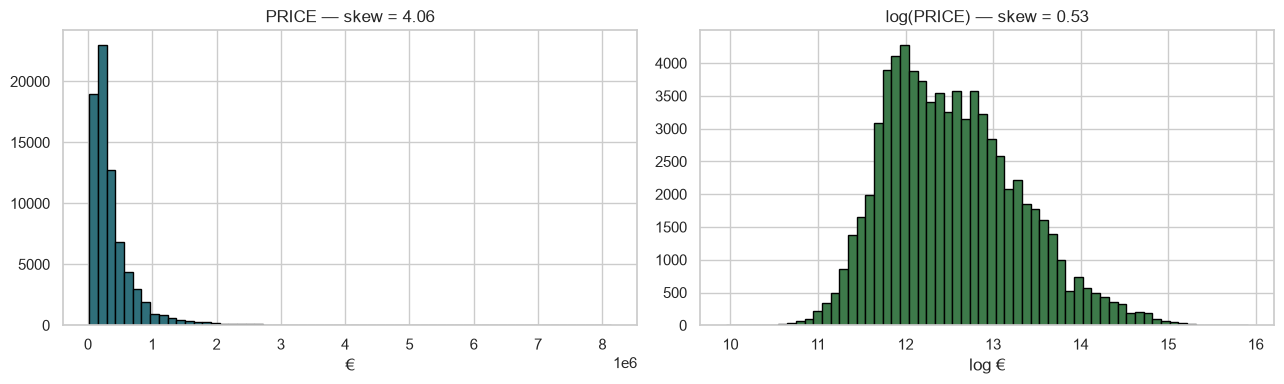
\includegraphics[width=0.8\linewidth]{nb01_distribucion_precio.png}
\caption{Distribución del precio anunciado en euros (izquierda) y en logaritmos (derecha). Fuente: cuaderno 01.}
\label{fig:distprecio}
\end{figure}

\paragraph{Fuga de información y variables ausentes.} El precio por metro cuadrado es exactamente el precio dividido por la superficie y se eliminó. Tampoco se usaron los campos sobre el precio de la plaza de garaje, que valen 1 € en el 99,96 \% de los casos y describen cómo se compone el precio, no la vivienda; sí se conserva el indicador de garaje. El año de construcción declarado falta en el 60 \% de los anuncios y se sustituyó por el catastral, que está completo. En las matrices de modelado, la planta (3,9 \% de ausentes) y la calidad catastral (un caso) se imputaron con valores calculados solo sobre los datos de entrenamiento.

\paragraph{Valores extremos.} No se eliminaron observaciones por sus valores extremos: las viviendas de las colas, como áticos grandes o pisos de lujo, son casos reales y no errores de medida, y su influencia queda acotada al trabajar en logaritmos.

\paragraph{Relaciones entre variables.} Las variables más correlacionadas con el precio (Spearman) son la superficie (0,72), la vulnerabilidad del barrio (0,71 en valor absoluto), el alquiler de barrio (0,67) y el número de baños (0,67). Entre las explicativas aparecen grupos esperables: las medidas de tamaño, las dos distancias de centralidad (0,77) y los dos indicadores socioeconómicos de barrio ($-0{,}76$). Ningún factor de inflación de la varianza supera 6, de modo que la colinealidad es moderada. Dos relaciones no lineales anticipan el capítulo siguiente: el año de construcción tiene forma de U, con los edificios históricos y la obra nueva más caros que los de los años sesenta y setenta, y la tasa de incidencias también, con los barrios de menor y mayor tasa como los más caros. Esta segunda relación desaparece al controlar por la centralidad, un ejemplo de por qué una asociación marginal no debe leerse como un efecto.

% ============================= 4 =============================
\section{Metodología}\label{sec:metodologia}

Este capítulo describe el proceso seguido desde el conjunto de trabajo hasta el modelo final: cómo se separaron los datos de entrenamiento y evaluación, qué forma funcional y qué variables se consideraron, qué familias de modelos se compararon y cómo se ajustaron sus hiperparámetros. El código y los resultados intermedios de cada paso están en los cuadernos 02 a 06 del repositorio [6].

\subsection{Partición de los datos y prevención de fugas}

Para el modelado, el conjunto se dividió aleatoriamente en entrenamiento (80 \%, 60.375 viviendas) y prueba (20 \%, 15.094 viviendas), con una semilla fija. Los parámetros de imputación, discretización y estandarización de las matrices finales se ajustaron sobre entrenamiento y se aplicaron después, sin cambios, a prueba. La selección de variables se realizó sobre entrenamiento mediante contribución al ajuste y BIC; la comparación de familias y la búsqueda de hiperparámetros utilizaron validación cruzada de cinco particiones dentro de ese conjunto. La evaluación final se realizó sobre las viviendas de prueba (capítulo~\ref{sec:resultados}).

La separación tiene una limitación: el análisis exploratorio y el estudio inicial de transformaciones de los cuadernos 01 y 02 examinaron el conjunto completo antes de construir las matrices de modelado. Por tanto, aunque el conjunto de prueba no se usó para ajustar los modelos ni sus hiperparámetros, no quedó aislado de todas las decisiones exploratorias. Una evaluación confirmatoria requeriría una muestra adicional reservada antes de explorar los datos.

La métrica de referencia durante todo el proceso es la raíz del error cuadrático medio sobre el logaritmo del precio (RMSE log). Al trabajar en logaritmos, esta métrica aproxima el error relativo típico de la predicción y trata por igual a viviendas baratas y caras, que es lo que interesa al comparar anuncios.

\subsection{Forma funcional de las variables}

Un modelo lineal aplicado directamente a las variables originales impone efectos aditivos y pendientes constantes, de modo que antes de decidir qué variables incluir es necesario decidir cómo entra cada una. El criterio utilizado fue la forma de la relación con el logaritmo del precio, no la forma de la distribución de la variable: para cada candidata se comparó el ajuste obtenido con la variable sin transformar, en logaritmos y discretizada en veinte cuantiles, que actúa como techo no paramétrico. Esta comparación mostró que la asimetría no es una buena guía. La tasa de incidencias, muy asimétrica, empeora al aplicarle logaritmos porque su relación con el precio tiene forma de U; el año de construcción, casi simétrico, multiplica su capacidad explicativa por más de diez al agruparlo por épocas constructivas.

Las decisiones resultantes fueron las siguientes. La superficie entra en logaritmos con un nudo en 50 m², porque por debajo de ese tamaño el precio por metro cuadrado se dispara y una única pendiente no representa ese tramo. El año de construcción se agrupa en épocas, con el periodo 1960--1975 como referencia; las habitaciones y la planta se discretizan en tramos, y las distancias al centro, a la Castellana y al metro entran en logaritmos. Estas transformaciones solo tienen sentido para la vía lineal. Un modelo de árboles es invariante a transformaciones monótonas y aprende por sí mismo umbrales e interacciones, por lo que para esa familia se utilizaron las variables sin transformar; lo único que comparten ambas vías es el logaritmo del precio como variable objetivo.

\subsection{Selección de variables}

Con más de 60.000 observaciones, prácticamente cualquier variable resulta estadísticamente significativa: en un modelo lineal con las 37 candidatas, 30 tienen un p-valor inferior a 0,05. La significación no sirve, por tanto, para decidir. En su lugar se utilizó el tamaño del efecto, medido como la contribución única de cada variable al $R^2$ (la pérdida de ajuste al retirarla del modelo completo) expresada como fracción de la varianza que el modelo aún no explica. El modelo completo alcanza un $R^2$ de 0,91, y se fijó un umbral del 1 \% de la varianza residual para considerar que el ajuste justifica por sí solo la inclusión.

El análisis muestra que el modelo descansa en muy pocas variables. La superficie explica por sí sola el 69 \% del $R^2$ del modelo completo; con el alquiler de barrio se alcanza el 95 \% y con nueve variables el 99 \% (Figura~\ref{fig:saturacion}). Agrupadas por bloques, el tamaño y la localización concentran prácticamente toda la contribución única, mientras que las características del edificio y los equipamientos explican bastante en solitario pero aportan poco una vez conocidos el tamaño y el barrio.

\begin{figure}[!htb]
\centering
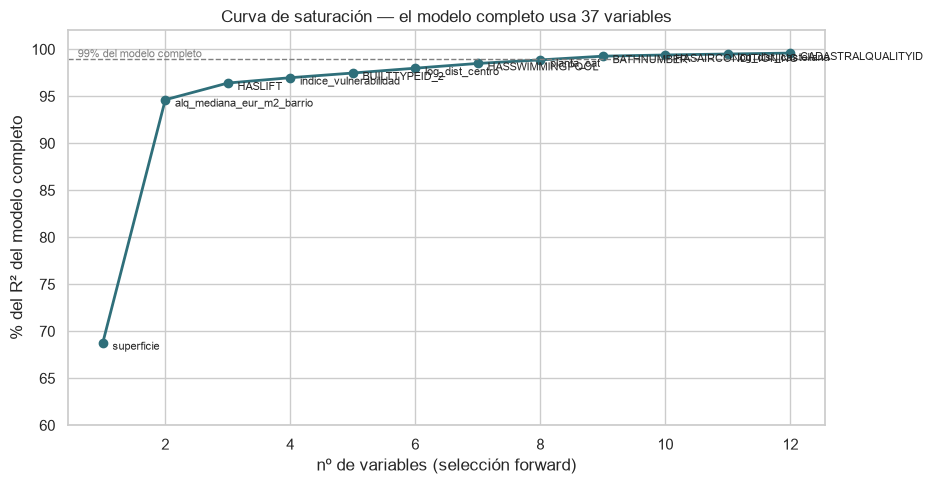
\includegraphics[width=0.9\linewidth]{nb03_saturacion.png}
\caption{Selección hacia delante en el modelo lineal: porcentaje del $R^2$ del modelo completo, con 37 variables, que se alcanza al añadir variables una a una. Fuente: cuaderno 03.}
\label{fig:saturacion}
\end{figure}

El ajuste no bastó en todos los casos, y varias decisiones se tomaron por razones de validez del dato:

\begin{itemize}[leftmargin=1.5em,itemsep=2pt,topsep=2pt]
\item \textbf{Distancias a equipamientos.} Sus valores típicos (150--500 m) son del mismo orden que el ruido de anonimización de las coordenadas, que llega a representar entre el 20 \% y el 64 \% de la distancia mediana. Las distancias al centro y a la Castellana, de varios kilómetros, no tienen ese problema. Se descartaron las primeras y se conservaron las segundas.
\item \textbf{Orientación.} Solo el 47 \% de los anuncios declara alguna, y un 18 \% declara más de una, de modo que un cero significa ``sin dato'' y no ``sin esa orientación''. Se descartó.
\item \textbf{Tasa de incidencias.} Su relación en U con el precio desaparece al controlar por el resto de variables: los residuos por quintil oscilan en torno a $\pm$1,5 \% sin patrón. Los barrios con más incidencias registradas son zonas céntricas y de ocio, que también son caras; la U reflejaba centralidad, no un efecto de la inseguridad.
\item \textbf{Variables catastrales.} El año de construcción, la calidad y la tipología catastral proceden de un cruce con la dirección exacta del inmueble, que un anuncio actual no proporciona. Se mantuvieron en el análisis, pero se construyó también una variante del conjunto de datos sin ellas.
\end{itemize}

Como comprobación independiente del umbral elegido, una selección por pasos con el criterio BIC retuvo 27 de las 37 variables y descartó igualmente las cuatro orientaciones. Conviene subrayar que esta poda se decidió sobre un modelo lineal aditivo: una variable irrelevante en ese contexto puede ser útil en un modelo de árboles a través de sus interacciones. Por ello, para los árboles se conservaron todas las variables salvo las descartadas por razones de validez, y el efecto de la poda se midió en lugar de darlo por supuesto.

\subsection{Variantes del conjunto de datos}

El resultado de las decisiones anteriores no es una única matriz de datos, sino varias variantes que permiten responder preguntas concretas. Las dos más relevantes son la variante \emph{completa}, con 28 variables incluidas las catastrales, y la variante \emph{desplegable}, con 21 variables, que prescinde de todo lo que no puede obtenerse de un anuncio actual: los campos catastrales, el número de viviendas del edificio y el indicador de última planta. La comparación entre ambas cuantifica cuánto cuesta, en precisión, que el modelo tenga que funcionar con la información disponible en producción. Se construyeron también variantes con la poda del apartado anterior y con las distancias a equipamientos y la orientación, para contrastar esas decisiones con cada familia de modelos.

\subsection{Comparación de familias de modelos}

Se compararon tres familias con hiperparámetros por defecto. La \textbf{regresión lineal} (MCO) es la referencia interpretable: sus coeficientes se leen directamente como efectos sobre el precio, y sería la opción preferida si su rendimiento fuera comparable al de las alternativas. \textbf{Random Forest} [13] promedia árboles entrenados sobre remuestreos de los datos, lo que reduce la varianza y captura no linealidades sin especificarlas. \textbf{XGBoost} [2] construye los árboles de forma secuencial, cada uno corrigiendo el error de los anteriores, e incorpora sus propios mecanismos de regularización.

\begin{table}[!htb]
\centering
\caption{RMSE log en validación cruzada (media de cinco particiones sobre el conjunto de entrenamiento).}
\label{tab:modelos}
\begin{tabularx}{\linewidth}{@{}L r r r r@{}}
\toprule
& \multicolumn{2}{c}{\thead{Por defecto}} & \multicolumn{2}{c}{\thead{Ajustado}} \\
\cmidrule(lr){2-3}\cmidrule(l){4-5}
\thead{Familia} & \thead{Completa} & \thead{Desplegable} & \thead{Completa} & \thead{Desplegable} \\
\midrule
Regresión lineal & 0,2277 & 0,2321 & -- & -- \\
Random Forest & 0,1880 & 0,1917 & 0,1832 & 0,1868 \\
XGBoost & 0,1944 & 0,1990 & \textbf{0,1801} & \textbf{0,1858} \\
\bottomrule
\end{tabularx}
\fuente{Fuente: elaboración propia (cuadernos 05 y 06). En la regresión lineal, las variantes corresponden al conjunto podado con y sin variables catastrales. La desviación típica entre particiones está entre 0,0015 y 0,0025.}
\end{table}

Los modelos de árboles superan con claridad a la regresión lineal (Tabla~\ref{tab:modelos}): su error es entre un 15 \% y un 17 \% menor, una diferencia muy superior a la variabilidad entre particiones, por lo que la familia lineal se descartó. Con los valores por defecto, Random Forest supera a XGBoost. Las variantes auxiliares confirmaron dos decisiones previas: añadir las distancias a equipamientos y la orientación empeora ligeramente el error (0,1899 frente a 0,1880 en Random Forest), mientras que aplicar la poda del modelo lineal tampoco mejora a los árboles (0,1889).

\subsection{Ajuste de hiperparámetros}

Antes de definir el espacio de búsqueda se diagnosticó el comportamiento de cada modelo por defecto, ya que un problema de varianza y uno de sesgo requieren ajustes en direcciones opuestas. En Random Forest, cada árbol alcanzaba una profundidad cercana a 40 niveles con apenas 1,6 observaciones por hoja, y el error en entrenamiento (0,069) era muy inferior al de validación (0,188): un problema claro de varianza, agravado porque todos los árboles consideraban todas las variables en cada división y estaban muy correlacionados entre sí. En XGBoost la situación era la contraria: el error de validación seguía bajando, aunque lentamente, mucho después de la iteración 100 y alcanzaba su mínimo en la 268 (Figura~\ref{fig:curvaxgb}), de modo que las 100 iteraciones por defecto dejaban el modelo \emph{infraentrenado}.

\begin{figure}[!htb]
\centering
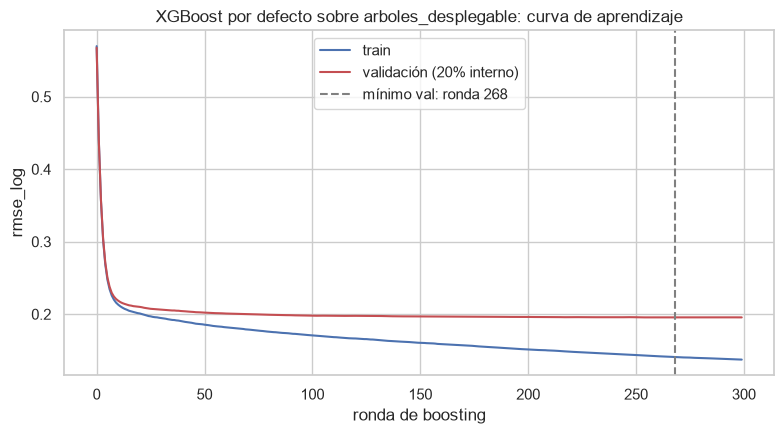
\includegraphics[width=0.55\linewidth]{nb06_curva_xgb.png}
\caption{Curva de aprendizaje de XGBoost con hiperparámetros por defecto sobre la variante desplegable, con un 20 \% del entrenamiento reservado para validación. Fuente: cuaderno 06.}
\label{fig:curvaxgb}
\end{figure}

Con este diagnóstico se realizó, para cada familia y variante, una búsqueda aleatoria de hiperparámetros con validación cruzada en dos etapas: una exploración amplia y un refinamiento centrado en la mejor región encontrada. Cada hiperparámetro de regularización incluía en su espacio el valor que lo desactiva, para que la búsqueda pudiera concluir que no era útil. En XGBoost la búsqueda se hizo con un número fijo de iteraciones y, una vez fijado el resto de hiperparámetros, el número de árboles se determinó con parada temprana en cada partición (sin mejora durante 50 iteraciones), tomando la mediana de las cinco particiones.

XGBoost obtuvo el mejor resultado en ambas variantes (Tabla~\ref{tab:modelos}), con una mejora del 7 \% respecto a su configuración por defecto, atribuible en buena parte a entrenar con suficientes iteraciones. De esta fase salen dos modelos. El \emph{ganador global} (variante completa, 835 árboles) indica el techo de precisión alcanzable con toda la información de 2018. El \emph{modelo de producción} (variante desplegable) es el que utiliza HabitIA: 410 árboles de profundidad máxima 12, tasa de aprendizaje 0,088, submuestreo del 96 \% de las filas y del 53 \% de las variables por árbol, y regularización L2 de 8,66. La configuración completa figura en el anexo~4.

\subsection{Retransformación a euros}

El modelo estima el logaritmo del precio. Aplicar la exponencial a esa estimación no recupera directamente la media en euros y puede introducir un sesgo a la baja. Para corregirlo se aplicó el estimador de \emph{smearing} de Duan [4], que no exige suponer normalidad en los residuos: la predicción en euros es $\hat{P} = e^{\hat{y}} \cdot s$, donde $s$ es la media de la exponencial de los residuos. Para que el factor no quedara subestimado, los residuos se calcularon fuera de muestra, con predicciones de validación cruzada sobre el conjunto de entrenamiento. El factor resultante es $s = 1{,}0168$ en el modelo de producción, lo que eleva las predicciones en torno a un 1,7 \%. Usar un único factor supone que la distribución de los residuos es suficientemente comparable entre viviendas; no corrige necesariamente el sesgo de todos los segmentos.

% ============================= 5 =============================
\section{Resultados}\label{sec:resultados}

Los dos modelos seleccionados se reentrenaron sobre todo el conjunto de entrenamiento y se evaluaron una única vez sobre las 15.094 viviendas de prueba. Este capítulo presenta su precisión, analiza dónde se concentran los errores y describe qué ha aprendido el modelo de producción.

\subsection{Precisión en el conjunto de prueba}

\begin{table}[!htb]
\centering
\caption{Resultados en el conjunto de prueba (precios anunciados de 2018).}
\label{tab:test}
\begin{tabularx}{\linewidth}{@{}L r r@{}}
\toprule
\thead{Métrica} & \thead{Ganador global} & \thead{Modelo de producción} \\
\midrule
RMSE log (validación cruzada) & 0,1801 & 0,1858 \\
RMSE log (prueba) & 0,1785 & 0,1856 \\
$R^2$ en logaritmos & 0,944 & 0,940 \\
Error absoluto medio / mediano & 45.774 € / 21.459 € & 49.220 € / 23.708 € \\
Error porcentual medio / mediano & 12,7 \% / 8,3 \% & 13,6 \% / 9,3 \% \\
Viviendas con error inferior al 10 \% & 57,4 \% & 52,8 \% \\
Viviendas con error inferior al 20 \% & 82,4 \% & 80,6 \% \\
Sesgo porcentual mediano & +1,0 \% & +1,0 \% \\
\bottomrule
\end{tabularx}
\end{table}

El modelo de producción comete un error porcentual mediano del 9,3 \%: para la mitad de las viviendas de prueba, la estimación se desvía menos de un 9,3 \% del precio anunciado, y cuatro de cada cinco quedan dentro de un margen del 20 \% (Tabla~\ref{tab:test}). El error medio en euros duplica al mediano, lo que indica que un grupo reducido de viviendas concentra errores grandes. El error en prueba es prácticamente igual al de validación cruzada en ambos modelos, señal de que la búsqueda de hiperparámetros no sobreajustó las particiones utilizadas. El sesgo mediano es ligeramente positivo, es decir, el modelo tiende a sobrestimar levemente.

Para comprobar si la diferencia entre ambos modelos es real, se generaron réplicas \emph{bootstrap} del conjunto de prueba y se calculó en cada una el error de los dos modelos sobre las mismas viviendas. Prescindir de las variables catastrales aumenta el RMSE log en 0,0071, con un intervalo de confianza al 95 \% de [0,0053; 0,0088], y el modelo de producción resulta peor en el 100 \% de las réplicas. La diferencia es, por tanto, real pero pequeña: aproximadamente un punto de error porcentual mediano. Es el precio de poder aplicar el modelo a anuncios actuales.

\subsection{Dónde se concentran los errores}

El error no se reparte por igual. Por nivel de precio, el decil más barato es claramente el más difícil (RMSE log de 0,27 y error mediano del 15,4 \%), seguido del más caro (0,20), mientras que los deciles centrales se sitúan en torno a 0,16. El modelo tiende a sobrestimar las viviendas más baratas, alrededor de un 8 \% en el quintil inferior, y a infraestimar ligeramente las más caras, un comportamiento habitual en modelos que regresan hacia la media. Por tamaño, el patrón es similar: los pisos de menos de 50 m² y los de más de 200 m² presentan más error que los intermedios. Por distritos, Centro es el más difícil para ambos modelos (0,20 y 0,21), probablemente por la heterogeneidad de su parque de viviendas, y Barajas el más sencillo (0,12). La Figura~\ref{fig:errorseg} resume ambos patrones.

\begin{figure}[!htb]
\centering
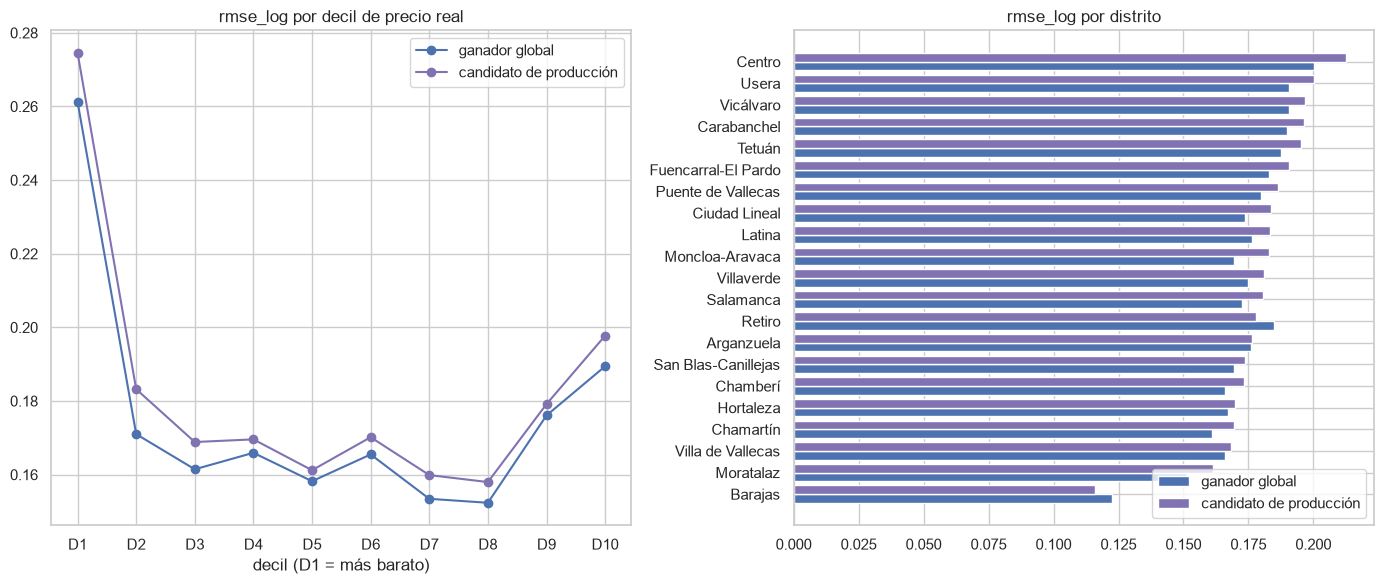
\includegraphics[width=0.85\linewidth]{nb07_error_segmentos.png}
\caption{RMSE log en el conjunto de prueba por decil de precio (izquierda) y por distrito (derecha), para el ganador global y el modelo de producción. Fuente: cuaderno 07.}
\label{fig:errorseg}
\end{figure}

La pérdida de las variables catastrales afecta sobre todo a las viviendas baratas y pequeñas: el aumento de error es de 0,013 en el decil inferior y de 0,010 en los pisos de menos de 50 m², frente a 0,003 en el decil 9. Es coherente con que la antigüedad y la calidad del edificio sirvan sobre todo para distinguir entre viviendas pequeñas de tamaño y barrio parecidos.

\subsection{Interpretación del modelo}

Para entender qué ha aprendido el modelo se calcularon los valores SHAP [12] de una muestra de 5.000 viviendas de prueba. Los valores SHAP descomponen cada predicción en la suma de una base común y una contribución por variable; como el modelo predice el logaritmo del precio, cada contribución se interpreta como un factor multiplicativo. La Figura~\ref{fig:shap} muestra el efecto típico de cada variable.

\begin{figure}[!htb]
\centering
\begin{tikzpicture}
\begin{axis}[
  xbar, y=0.42cm, enlarge y limits=0.06,
  xmin=0, xmax=40, width=12cm,
  bar width=7pt,
  xlabel={\footnotesize Efecto típico sobre el precio estimado (\%)},
  symbolic y coords={Incidencias,Garaje,Piscina,Aire acondicionado,Distancia a Castellana,Planta,Distancia al centro,Ascensor,Baños,Vulnerabilidad,Alquiler de barrio,Superficie},
  ytick=data, tick label style={font=\scriptsize},
  nodes near coords, nodes near coords align={horizontal},
  every node near coord/.append style={font=\scriptsize},
  nodes near coords={\pgfmathprintnumber[fixed,precision=1,use comma]{\pgfplotspointmeta}},
  point meta=explicit,
]
\addplot[fill=blue!35!black,draw=blue!35!black] coordinates {
  (34.3,Superficie)[34.3]
  (18.0,Alquiler de barrio)[18.0]
  (11.2,Vulnerabilidad)[11.2]
  (6.9,Baños)[6.9]
  (6.3,Ascensor)[6.3]
  (5.1,Distancia al centro)[5.1]
  (3.6,Planta)[3.6]
  (3.5,Distancia a Castellana)[3.5]
  (2.5,Aire acondicionado)[2.5]
  (2.2,Piscina)[2.2]
  (1.9,Garaje)[1.9]
  (1.9,Incidencias)[1.9]};
\end{axis}
\end{tikzpicture}
\caption{Efecto típico de las doce variables más influyentes del modelo de producción, calculado como $e^{\text{media}|\phi|}-1$ sobre 5.000 viviendas de prueba.}
\label{fig:shap}
\end{figure}

La superficie es, con diferencia, la variable más influyente, seguida de los dos indicadores socioeconómicos del barrio. Las tres variables de localización (alquiler, vulnerabilidad y distancia al centro) tienen en conjunto un peso comparable al de la superficie: el precio depende en medida parecida de cuánta vivienda se compra y de dónde está. Entre los equipamientos destaca el ascensor: las viviendas que lo tienen reciben, de media, una contribución un 14,9 \% superior a las que no. Le siguen la piscina (9,0 \%), el garaje (5,8 \%) y el aire acondicionado (5,2 \%); el resto de equipamientos aporta menos de un 3,5 \%. Al comparar con el ganador global se observa que, sin las variables catastrales, el número de baños y el ascensor ganan peso: el modelo los utiliza en parte como aproximación a la antigüedad y la calidad del edificio.

Estos resultados deben leerse con tres precauciones. Explican el comportamiento del modelo, no el del mercado, por lo que no son efectos causales. Con variables correlacionadas, el reparto de la contribución entre ellas es en parte arbitrario. Y la comparación de equipamientos enfrenta a viviendas distintas, no a la misma vivienda con y sin el equipamiento. El apartado siguiente examina precisamente qué ocurre al cambiar una característica de una misma vivienda.

\subsection{Sensibilidad del modelo}

Los valores SHAP también permiten ver cómo cambia la contribución de una variable a lo largo de su rango. En la Figura~\ref{fig:dependencia}, cada punto es una vivienda de prueba y su altura indica cuánto modifica esa variable su precio estimado. Las formas son coherentes con lo esperable. El efecto de la superficie es creciente y más que proporcional por encima de unos 100 m², mientras que los pisos pequeños tienen un precio por metro cuadrado mayor. El alquiler de barrio y la vulnerabilidad desplazan la estimación entre un $-30$ \% y un $+30$ \% y entre un $+20$ \% y un $-20$ \%, respectivamente. La cercanía al centro solo añade valor en los primeros tres kilómetros, cada baño adicional suma entre un 5 \% y un 10 \% hasta el cuarto, y los sótanos y bajos restan entre un 10 \% y un 20 \% frente a las plantas altas.

\begin{figure}[!htb]
\centering
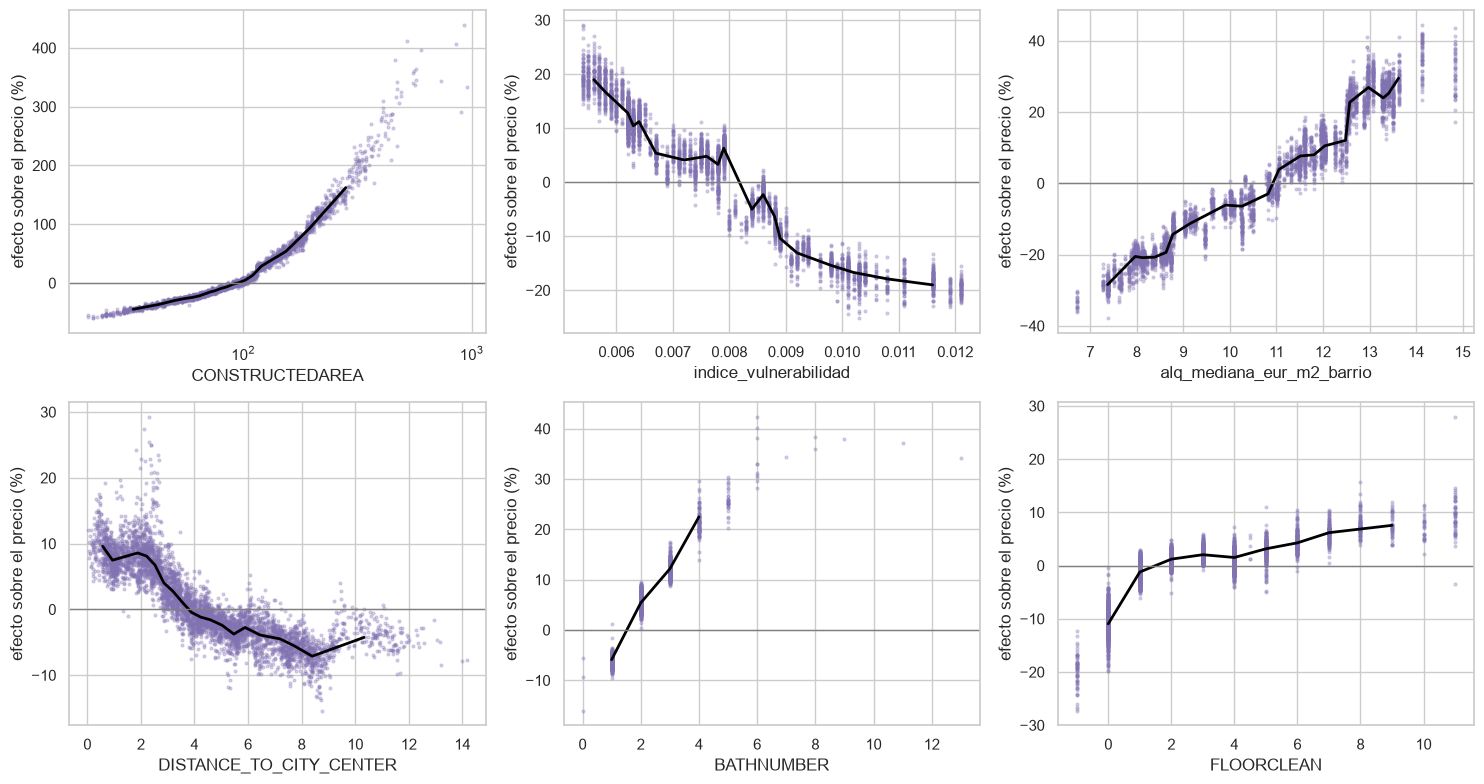
\includegraphics[width=0.85\linewidth]{nb07_dependencia_shap.png}
\caption{Contribución SHAP de seis variables al precio estimado por el modelo de producción, sobre 5.000 viviendas de prueba. La línea negra es la media por tramos. Fuente: cuaderno 07.}
\label{fig:dependencia}
\end{figure}

La vista complementaria consiste en tomar una vivienda y cambiar una sola de sus características. La Tabla~\ref{tab:sensibilidad} lo hace sobre el piso de ejemplo del capítulo~\ref{sec:produccion} (80 m², dos habitaciones, un baño, segunda planta, con ascensor y garaje, en el entorno de Sol). La ubicación es, con diferencia, lo que más mueve la estimación: el mismo piso vale un 38 \% más en Salamanca y un 55 \% menos en Villaverde. La planta y la descripción del anuncio tienen efectos intermedios, del orden de las cifras de la Figura~\ref{fig:dependencia}.

\begin{table}[!htb]
\centering
\caption{Variación del precio estimado (2018) al cambiar una característica del piso de ejemplo, cuya estimación base es de 324.654 €.}
\label{tab:sensibilidad}
\begin{tabularx}{\linewidth}{@{}L r L r@{}}
\toprule
\thead{Cambio} & \thead{Variación} & \thead{Cambio} & \thead{Variación} \\
\midrule
Planta baja & $-23{,}1$ \% & Ubicación en Salamanca & $+38{,}4$ \% \\
Primera planta & $-16{,}8$ \% & Ubicación en Chamberí & $+33{,}4$ \% \\
Octava planta & $+13{,}4$ \% & Ubicación en Tetuán & $+18{,}8$ \% \\
Dos baños & $+10{,}1$ \% & Ubicación en Carabanchel & $-36{,}3$ \% \\
Sin ascensor & $-4{,}9$ \% & Ubicación en Puente de Vallecas & $-37{,}4$ \% \\
Sin descripción (equipamientos) & $-15{,}8$ \% & Ubicación en Villaverde & $-55{,}0$ \% \\
Sin garaje & $+8{,}9$ \% & Tres habitaciones & $-25{,}2$ \% \\
\bottomrule
\end{tabularx}
\fuente{Fuente: elaboración propia con el paquete de producción. Las variaciones de ubicación no incluyen el índice de distrito.}
\end{table}

Dos resultados muestran el límite de este tipo de lectura. Quitar el garaje eleva la estimación un 8,9 \%, y pasar de dos a tres habitaciones sin cambiar la superficie la reduce un 25 \%. El modelo reproduce asociaciones entre viviendas distintas (con la superficie fija, más habitaciones suele significar estancias pequeñas en edificios antiguos), no el efecto de añadir o quitar algo a una misma vivienda. Los árboles aprenden umbrales, y la función resultante es escalonada y no necesariamente monótona. En consecuencia, el modelo es adecuado para comparar anuncios tal como se publican, pero no para simular reformas o ampliaciones.

\begin{figure}[!htb]
\centering
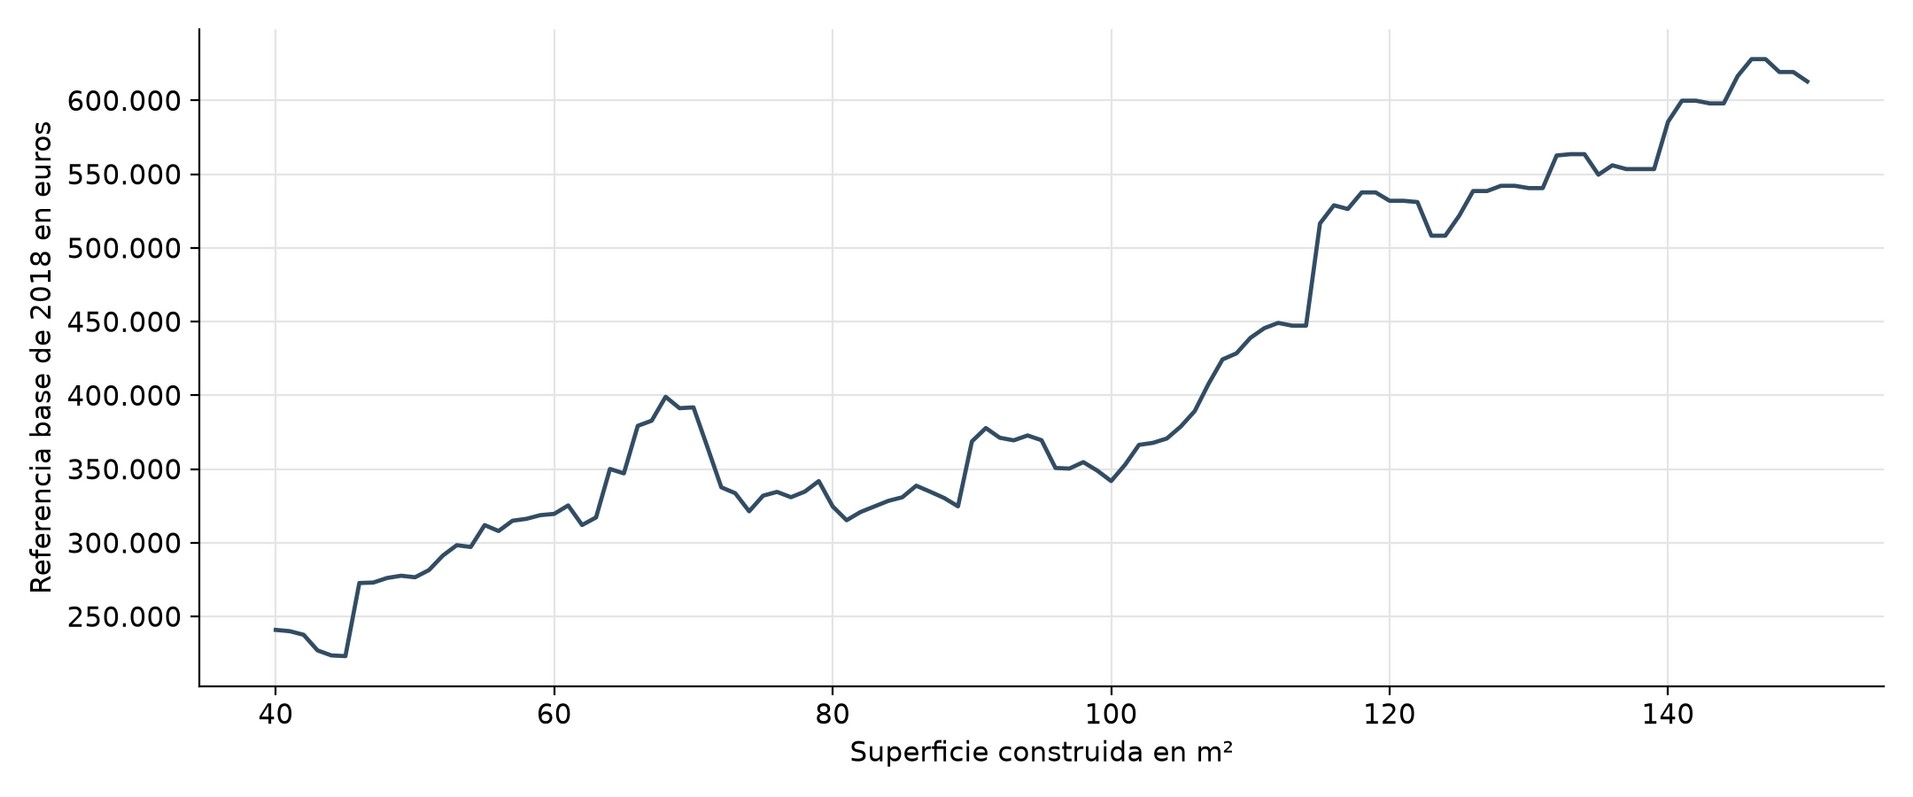
\includegraphics[width=0.65\linewidth]{sensibilidad_superficie.png}
\caption{Precio estimado a precios de 2018 del piso de ejemplo al variar solo su superficie entre 40 y 150 m².}
\label{fig:sensarea}
\end{figure}

% ============================= 6 =============================
\section{Del modelo a producción}\label{sec:produccion}

El modelo aprendió a partir de anuncios de 2018 descritos con un conjunto de variables concreto. Aplicarlo a un anuncio publicado hoy exige resolver dos problemas: reconstruir esas mismas variables a partir de la información que ofrece la API de Idealista, y trasladar una estimación con precios de 2018 al nivel de precios actual. Este capítulo describe ambos pasos, el dominio en el que el modelo se considera aplicable y un contraste con anuncios reales de 2026. El proceso está documentado en el cuaderno 08 [6].

\subsection{Reconstrucción de las variables}

Las características básicas (superficie, habitaciones, baños, planta, ascensor, garaje y tipología) se leen directamente de los campos del anuncio; cuando la planta falta, se imputa con la mediana de entrenamiento. Las tres distancias se recalculan con la fórmula de haversine sobre los mismos puntos de referencia de \emph{idealista18}; aplicado a 5.000 anuncios de 2018, este cálculo reproduce las distancias originales con un error mediano inferior a 5 metros. El barrio se asigna por cruce espacial, con la misma cartografía, y recupera el barrio de entrenamiento en el 99,1 \% de los anuncios de 2018.

La API no informa de siete equipamientos (terraza, aire acondicionado, trastero, armarios empotrados, piscina, portero y jardín), que se extraen de la descripción mediante reglas de texto. Cada equipamiento se clasifica como mencionado, negado o sin mención, y solo el primer caso cuenta como presente. Las reglas incluyen exclusiones para los falsos positivos más frecuentes, como la ``piscina municipal cercana'', el ``portero automático'' o la ``preinstalación de aire acondicionado''. Esta extracción tiene una limitación evidente: un equipamiento que el anunciante no menciona se considera ausente. En el caso de ejemplo del apartado siguiente, eliminar la descripción reduce la estimación un 15,8 \%.

Las variables de barrio requieren un tratamiento específico. El índice de vulnerabilidad y la tasa de incidencias se construyeron para el entrenamiento con fuentes municipales, por lo que se reutilizan los mismos valores. El alquiler de barrio, en cambio, ha subido desde 2018 y utilizar su valor actual haría que cualquier vivienda pareciera estar en un barrio más caro de lo que el modelo conoce; además, esa subida se contaría dos veces al aplicar después el índice de precios. Por ello, el alquiler actual de cada barrio se divide por la subida media del alquiler en la ciudad y se aplica un factor de calibración que corrige las diferencias de método con el valor de entrenamiento. De este modo, la variable solo cambia en los barrios cuyo alquiler ha evolucionado más o menos deprisa que el conjunto de la ciudad.

\subsection{Actualización de precios a 2026}

La predicción del modelo es un precio anunciado de 2018. Para llevarla al nivel actual se aplica un índice de precios de venta por distrito, construido con la estadística registral de compraventas del Ayuntamiento:
\begin{equation*}
\hat{P}_{2018} = e^{\hat{y}} \cdot s, \qquad \hat{P}_{2026} = \hat{P}_{2018} \cdot I_d, \qquad I_d = \frac{V_{d,2026}}{V_{d,2018}},
\end{equation*}
donde $V_{d,t}$ es el precio medio por metro cuadrado del distrito $d$ en el año $t$. Se utiliza el distrito y no el barrio porque la serie por barrio tiene muy pocas operaciones en algunas zonas y resulta demasiado ruidosa. Como la serie de venta termina en 2025, el valor de 2026 se proyecta con la tendencia log-lineal de cada distrito desde 2018, que en el distrito mediano equivale a un crecimiento del 6,4 \% anual. Los índices resultantes oscilan entre 1,48 en Barajas y 2,26 en Vicálvaro.

Para las búsquedas de alquiler, la aplicación necesita además una referencia de renta mensual. Se obtiene multiplicando el precio de venta estimado por la relación entre alquiler y precio de venta del distrito en 2026, $\hat{R}_{2026} = \hat{P}_{2026} \cdot q_d$, con el alquiler proyectado igualmente desde su último dato, de 2024. Es importante distinguir ambas cifras: la estimación de venta procede de un modelo evaluado, mientras que la renta es una derivación a partir de ratios territoriales que no se ha podido validar de forma independiente.

Como ejemplo, un piso sintético de 80 m² en el distrito Centro, con dos habitaciones, un baño, ascensor y garaje, y cuya descripción menciona terraza, aire acondicionado, armarios empotrados y trastero, recibe una estimación de 324.654 € a precios de 2018. Con el índice de Centro (1,559) su referencia actual es de 506.053 €, y la renta mensual derivada es de 1.278 €. Si se anuncia en venta por 450.000 €, su precio queda un 11,1 \% por debajo de la referencia.

\subsection{Dominio de aplicación}

No todos los anuncios pueden valorarse con garantías, y en esos casos el sistema se abstiene en lugar de ofrecer una cifra engañosa. Se excluyen las casas y chalets, porque el modelo no dispone de información sobre la parcela; las viviendas de más de 367 m², mediante un límite conservador fijado en el percentil 99 del entrenamiento para evitar la escasa representación de superficies extremas; y las viviendas a reformar u ocupadas, detectadas en la descripción, porque el modelo no conoce el estado de conservación ni la situación de la posesión y las valoraría como si estuvieran en condiciones normales. Otras situaciones no bloquean la valoración pero se advierten: variables fuera del rango de entrenamiento, planta imputada o viviendas de obra nueva, cuyos anuncios de una misma promoción no son observaciones independientes.

\subsection{Contraste con anuncios de 2026}

Para observar el comportamiento del sistema en condiciones reales se descargaron 500 anuncios de venta de Madrid a través de la API de Idealista, seleccionando páginas de resultados al azar para evitar el sesgo de los anuncios destacados, que en una primera descarga eran casi todos de lujo. De ellos, 88 quedaron fuera del dominio y 412 se valoraron. La mediana del cociente entre precio anunciado y estimación es de 1,003, lo que indica un cociente típico cercano a uno en esta muestra, sin demostrar ausencia de sesgo en todo el mercado. El error porcentual absoluto mediano respecto al precio anunciado es del 12,9 \% y el 68,4 \% de los anuncios queda dentro de un margen del 20 \% (Figura~\ref{fig:anunciado}).

Estas cifras miden la desviación respecto al precio anunciado en esa muestra, como las métricas históricas, pero no validan el valor de cierre ni proceden de una nueva prueba reservada. Su orden de magnitud es razonable: el 12,9 \% es mayor que el 9,3 \% del conjunto de prueba, calculado con el mismo denominador (el precio anunciado), como cabe esperar al sumar la incertidumbre de la proyección de precios y de la extracción de variables desde texto. El contraste también revela patrones que el modelo no puede captar: los áticos se anuncian en torno a un 12 \% por encima de la estimación y las viviendas de obra nueva un 9 \% por debajo, aunque ambos grupos son pequeños.

\begin{figure}[!htb]
\centering
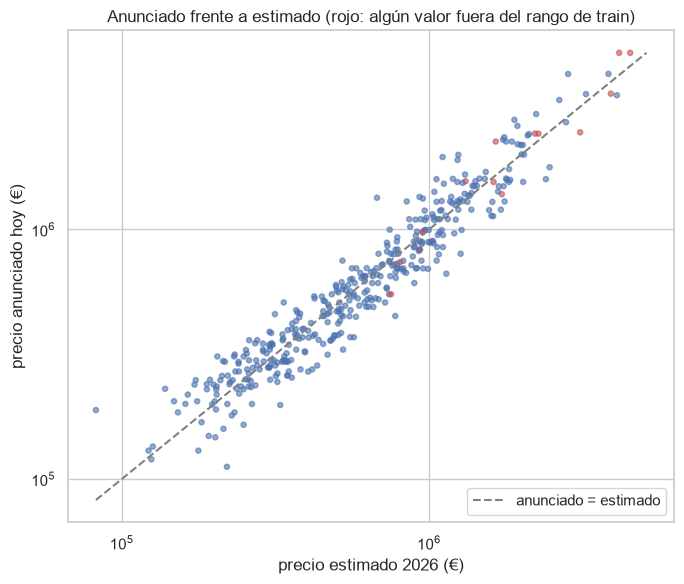
\includegraphics[width=0.6\linewidth]{nb08_anunciado_estimado.png}
\caption{Precio anunciado frente a precio estimado en 2026 para 412 anuncios de venta, en escala logarítmica. En rojo, anuncios con alguna variable fuera del rango de entrenamiento. Fuente: cuaderno 08.}
\label{fig:anunciado}
\end{figure}

\newpage
% ============================= 7 =============================
\section{La aplicación HabitIA}\label{sec:aplicacion}

HabitIA traslada el modelo a una herramienta de búsqueda y comparación de vivienda en Madrid capital. La persona usuaria puede buscar mediante filtros o describir lo que necesita a un asistente conversacional, y en ambos casos obtiene anuncios reales acompañados de una referencia de precio y de una puntuación adaptada a sus preferencias. Este capítulo describe la arquitectura del sistema, el recorrido de una búsqueda, el diseño del asistente conversacional y la puntuación con la que se ordenan los resultados. El detalle técnico de la integración, el formato de entrada y salida del servicio de inferencia y las pruebas realizadas se recogen en el anexo~14.

\subsection{Arquitectura}

El sistema separa la aplicación web, desarrollada en Next.js y publicada en Vercel, del servicio de inferencia, desarrollado en Python con FastAPI y desplegado en Fly.io (Figura~\ref{fig:arquitectura}). Esta separación responde a una razón práctica: el modelo necesita XGBoost, bibliotecas geoespaciales y varios artefactos de datos que no conviene empaquetar en cada función de la aplicación web. El servicio de inferencia contiene el modelo y las tablas territoriales necesarias para reconstruir las variables, y verifica al arrancar la integridad de todos ellos. La aplicación web concentra la lógica de búsqueda, la consulta a proveedores externos (Idealista, geocodificación y cálculo de trayectos), la persistencia en Supabase y el agente conversacional. Las credenciales permanecen siempre en el servidor, y el navegador solo recibe resultados.

\begin{figure}[!htb]
\centering
\resizebox{0.95\linewidth}{!}{%
\begin{tikzpicture}[>={Stealth[]},
  blk/.style={draw,rounded corners=2pt,align=center,text width=4cm,minimum height=1.25cm,fill=gray!6,font=\footnotesize},
  node distance=8mm and 16mm]
\node[blk] (nav) {\textbf{Navegador}\\[2pt]\scriptsize Interfaz React\\ Perfil y última búsqueda};
\node[blk,right=of nav] (web) {\textbf{Servidor web}\\[2pt]\scriptsize Next.js en Vercel\\ API y validación};
\node[blk,right=of web] (ag) {\textbf{Agente conversacional}\\[2pt]\scriptsize Anthropic y herramientas\\ Interpretación y texto};
\node[blk,below=1.1cm of web] (log) {\textbf{Lógica de aplicación}\\[2pt]\scriptsize Búsqueda y enriquecimiento\\ Comparación y preferencias};
\node[blk,below=1.1cm of nav] (prov) {\textbf{Proveedores}\\[2pt]\scriptsize Idealista y contexto\\ Geocodificación y trayectos};
\node[blk,below=1.1cm of log] (per) {\textbf{Persistencia}\\[2pt]\scriptsize Supabase\\ Cachés y demo compartida};
\node[blk,below=1.1cm of ag] (inf) {\textbf{Servicio de inferencia}\\[2pt]\scriptsize FastAPI en Fly.io\\ XGBoost y tablas};
\draw[->] (nav)--(web) node[midway,above,font=\tiny]{HTTPS};
\draw[->] (web)--(ag);
\draw[->] (web)--(log);
\draw[->] (ag)--(log) node[midway,above right,font=\tiny,inner sep=1pt]{herramientas};
\draw[->] (log)--(prov);
\draw[->] (log)--(per);
\draw[->] (log)--(inf) node[midway,below,font=\tiny]{HTTPS y token};
\end{tikzpicture}}
\caption{Componentes principales de HabitIA. Las flechas representan llamadas; las respuestas recorren el camino inverso.}
\label{fig:arquitectura}
\end{figure}

\newpage

\subsection{Recorrido de una búsqueda}

La búsqueda comienza en la portada, donde se elige la operación (compra o alquiler) y la zona. El perfil permite concretar presupuesto, número de habitaciones, requisitos imprescindibles y el lugar habitual de desplazamiento, como el trabajo. Antes de lanzar la búsqueda, el panel muestra los filtros para que la persona los confirme; esta separación evita consumir consultas a Idealista de forma involuntaria. El servidor comprueba entonces que la zona pertenece a Madrid capital y rechaza cualquier otra ubicación.

Si existe una respuesta reciente para la misma consulta, se reutiliza desde una caché de 24 horas; en caso contrario, se consulta la API de Idealista. Los anuncios obtenidos se filtran por presupuesto, habitaciones e imprescindibles. Un imprescindible solo excluye un anuncio cuando consta que no se cumple: si el anuncio no dice nada, se mantiene como desconocido. Los candidatos se envían en bloque al servicio de inferencia, que devuelve para cada uno su referencia de precio o el motivo por el que no puede valorarse, y se calcula el tiempo de trayecto hasta el lugar indicado. Finalmente, los resultados se ordenan según la puntuación descrita a continuación y se muestran los cinco mejores, con una explicación de por qué encajan.

\subsection{Asistente conversacional}

El asistente ofrece las mismas capacidades que el buscador a través de una conversación en lenguaje natural. Utiliza un modelo de lenguaje de Anthropic (Claude Opus 4.6, configurable) mediante la API de mensajes con uso de herramientas (\emph{tool use}) y respuesta en streaming. El principio de diseño es una división estricta de funciones: el modelo de lenguaje interpreta la petición, decide qué herramientas llamar y redacta la respuesta, pero no calcula ninguna cifra. Precios, estimaciones, trayectos y simulaciones proceden siempre de herramientas deterministas, las mismas que utiliza el buscador. Esta separación reduce el riesgo de que el modelo genere un precio o un porcentaje plausible pero inventado, aunque la fidelidad del texto a los resultados requiere evaluación.

\begin{table}[!htb]
\centering
\caption{Herramientas disponibles para el asistente.}
\label{tab:herramientas}
\begin{tabularx}{\linewidth}{@{}l L@{}}
\toprule
\thead{Herramienta} & \thead{Función} \\
\midrule
buscar\_propiedades & Busca anuncios en Idealista dentro de Madrid capital según zona, operación, precio, superficie y habitaciones \\
detalle\_propiedad & Recupera la información disponible de un anuncio ya mostrado \\
valorar\_vivienda & Llama al servicio de inferencia con los datos observados del anuncio y devuelve la estimación, la comparación y las advertencias \\
valorar\_alquiler & Consulta una referencia territorial de renta por metro cuadrado \\
analizar\_mercado & Compara el precio por metro cuadrado con la media provincial del INE y aporta el tipo hipotecario del Banco de España \\
calcular\_hipoteca & Calcula cuota mensual, coste total y esfuerzo sobre el salario \\
calcular\_trayecto & Estima el tiempo desde el lugar de trabajo a pie, en bici, en coche y en transporte público \\
comparar\_alquiler\_compra & Simula año a año el patrimonio de comprar frente a alquilar e invertir \\
consultar\_barrio & Informa de la disponibilidad de indicadores de barrio sin clasificar zonas \\
\bottomrule
\end{tabularx}
\end{table}

Cada petición sigue un bucle de agente. El servidor envía al modelo la conversación, las instrucciones del sistema y la definición de las nueve herramientas de la Tabla~\ref{tab:herramientas}, descritas en español y orientadas a \emph{cuándo} conviene usar cada una. Si el modelo solicita herramientas, el servidor las ejecuta, devuelve sus resultados y vuelve a llamar al modelo, que puede encadenar nuevas llamadas o responder. Un recorrido típico ante una petición como ``busco un piso de dos habitaciones en Chamberí para comprar, hasta 500.000 €'' consiste en buscar anuncios, valorar los más relevantes con el modelo y, si el perfil incluye un lugar de trabajo, calcular el trayecto. Para acotar la latencia y el coste, cada petición admite como máximo tres llamadas al modelo y cuatro ejecuciones de herramientas, con tiempos límite de 45 segundos por llamada y 52 segundos en total. Si una herramienta falla, el error se devuelve al modelo como resultado marcado, de forma que pueda explicarlo en lugar de continuar como si tuviera datos.

Cada herramienta produce dos representaciones de su resultado. El modelo recibe una versión compacta: la búsqueda, por ejemplo, le devuelve un resumen sin la lista completa de anuncios, lo que reduce el consumo de tokens. La interfaz recibe la versión completa y la muestra como tarjetas (anuncios, valoración, hipoteca, trayecto o mercado), que llegan al navegador como eventos de servidor mientras el texto se genera. Las cifras que ve la persona usuaria son, por tanto, las de la herramienta y no las de la redacción del modelo.

El servidor no guarda estado entre peticiones: el navegador reenvía el historial, limitado a 20 mensajes y 32.000 caracteres. Para que el asistente pueda valorar más adelante un anuncio mostrado en un turno anterior sin inventar sus coordenadas ni sus características, los datos observados de esos anuncios se adjuntan al historial como contenido estructurado. El perfil de la persona usuaria (operación, zona, presupuesto, trabajo y pesos de la puntuación) se incorpora a las instrucciones del sistema para no volver a preguntar lo que ya se conoce.

Las instrucciones del sistema fijan el comportamiento en cuatro aspectos. En la recogida de información, el asistente necesita zona, presupuesto y operación antes de buscar, y no hace más de dos preguntas por turno. En el ámbito, solo busca en Madrid capital y no ofrece asesoramiento legal ni fiscal. En el uso de la evidencia, debe indicar el periodo de la estimación, explicar las abstenciones del modelo y no inventar intervalos, puntuaciones ni valores que las herramientas no hayan devuelto. En seguridad, los campos del perfil y de los anuncios se tratan como datos y nunca como instrucciones, una defensa básica frente a la inyección de instrucciones a través del texto de un anuncio. A nivel de servidor, las peticiones se validan, se limitan por dirección IP y el asistente puede desactivarse con una variable de entorno para controlar el consumo.

El buscador utiliza también un modelo de lenguaje, más rápido (Claude Sonnet 4.6), para redactar opcionalmente una frase que explique por qué encaja cada vivienda a partir de los datos ya calculados; si la llamada falla o tarda más de 15 segundos, se mantiene la explicación determinista. El comportamiento del asistente no se ha evaluado de forma sistemática, por ejemplo midiendo el acierto en la elección de herramientas o la fidelidad de las respuestas a sus resultados, y esa evaluación queda como trabajo futuro.

\hfill

\begin{figure}[!htb]
\centering
\begin{tikzpicture}[>={Stealth[]},node distance=6mm,
  paso/.style={draw,rounded corners=2pt,align=center,text width=10.5cm,minimum height=0.9cm,fill=gray!6,font=\small}]
\node[paso] (peticion) {Petición de la persona y datos del perfil};
\node[paso,below=of peticion] (agente) {El asistente selecciona una herramienta y sus parámetros};
\node[paso,below=of agente] (herramienta) {El servidor ejecuta la consulta o el cálculo};
\node[paso,below=of herramienta] (resultado) {Resultado completo: tarjetas de la interfaz\\Resumen del resultado: contexto para el asistente};
\node[paso,below=of resultado] (texto) {El asistente explica el resultado o solicita otra herramienta};
\draw[->] (peticion)--(agente);
\draw[->] (agente)--(herramienta);
\draw[->] (herramienta)--(resultado);
\draw[->] (resultado)--(texto);
\end{tikzpicture}
\caption{Flujo del asistente: la herramienta proporciona los datos de las tarjetas y el modelo de lenguaje redacta su explicación.}
\label{fig:chat}
\end{figure}


\subsection{Puntuación y presentación de resultados}

Cada anuncio recibe una puntuación de 0 a 100, el HabitIA Score, que suma cuatro componentes ponderados con pesos enteros elegidos por la persona usuaria, que suman 100 (25 cada uno por defecto):
\begin{equation*}
\text{Score} = \frac{\alpha \cdot \text{Fair} + \beta \cdot \text{Opportunity} + \gamma \cdot \text{Zone} + \delta \cdot \text{Lifestyle}}{100}.
\end{equation*}
La Tabla~\ref{tab:score} define cada componente. Presupuesto, habitaciones e imprescindibles no forman parte de la puntuación, sino que actúan como filtros previos.

\begin{table}[!htb]
\centering
\caption{Componentes del HabitIA Score.}
\label{tab:score}
\begin{tabularx}{\linewidth}{@{}l L L@{}}
\toprule
\thead{Componente} & \thead{Qué mide} & \thead{Cálculo (acotado entre 0 y 100)} \\
\midrule
Fair & Precio pedido frente a la referencia del modelo & $50 - 2{,}5\,b$, con $b$ la desviación porcentual del precio anunciado respecto a la referencia \\
Opportunity & Evolución reciente de los precios del distrito & $50 + 2{,}5\,(g_d - g_M)$, con $g$ la variación interanual del precio de oferta publicada por Idealista para el distrito y para Madrid (agosto de 2025 a agosto de 2026) \\
Zone & Dotaciones del distrito & Media de los rangos percentiles del distrito entre los 21 de Madrid en superficie de zonas verdes, líneas de metro y locales de servicios, y en actuaciones policiales (en sentido inverso) \\
Lifestyle & Tiempo de trayecto al trabajo & 100 hasta 10 minutos, 1,9 puntos menos por minuto adicional y 5 a partir de 60 minutos \\
\bottomrule
\end{tabularx}
\end{table}

Con estas escalas, un anuncio al precio de referencia obtiene 50 puntos en Fair, uno un 20 \% por debajo obtiene 100 y uno un 20 \% por encima, 0. Cuando un componente no puede calcularse, por ejemplo porque el modelo se abstiene o no se ha indicado un lugar de trabajo, aporta cero puntos y su peso no se reparte entre los demás. La interfaz lo señala como una puntuación parcial e indica qué fracción ha podido calcularse, para que un valor bajo por falta de datos no se confunda con una mala valoración.

La puntuación es una heurística de ordenación y no un resultado validado, y sus componentes tienen un fundamento desigual. Fair y Lifestyle dependen de la vivienda concreta y tienen una lectura directa. Opportunity y Zone, en cambio, se calculan por distrito, de modo que toman el mismo valor para todos los anuncios de una búsqueda en una misma zona y apenas alteran el orden dentro de ella. Sus definiciones son además discutibles. Opportunity premia los distritos cuyo precio de oferta más ha subido en el último año, lo que refleja inercia de precios más que oportunidad y puede entrar en tensión con Fair; como la referencia de Madrid (2,2 \%) queda por debajo de 19 de los 21 distritos, la mayoría supera los 50 puntos. Zone usa recuentos absolutos, sin normalizar por superficie ni población, lo que favorece a los distritos extensos en zonas verdes y penaliza a los céntricos, con más actividad, en actuaciones policiales. Una revisión de ambos componentes con indicadores relativos y a escala de barrio o del entorno de cada vivienda se plantea en el capítulo de conclusiones.

\hfill

\begin{figure}[!htb]
\centering

\includegraphics[width=0.9\linewidth]{app_inicio.png}
\par\vspace{8pt}
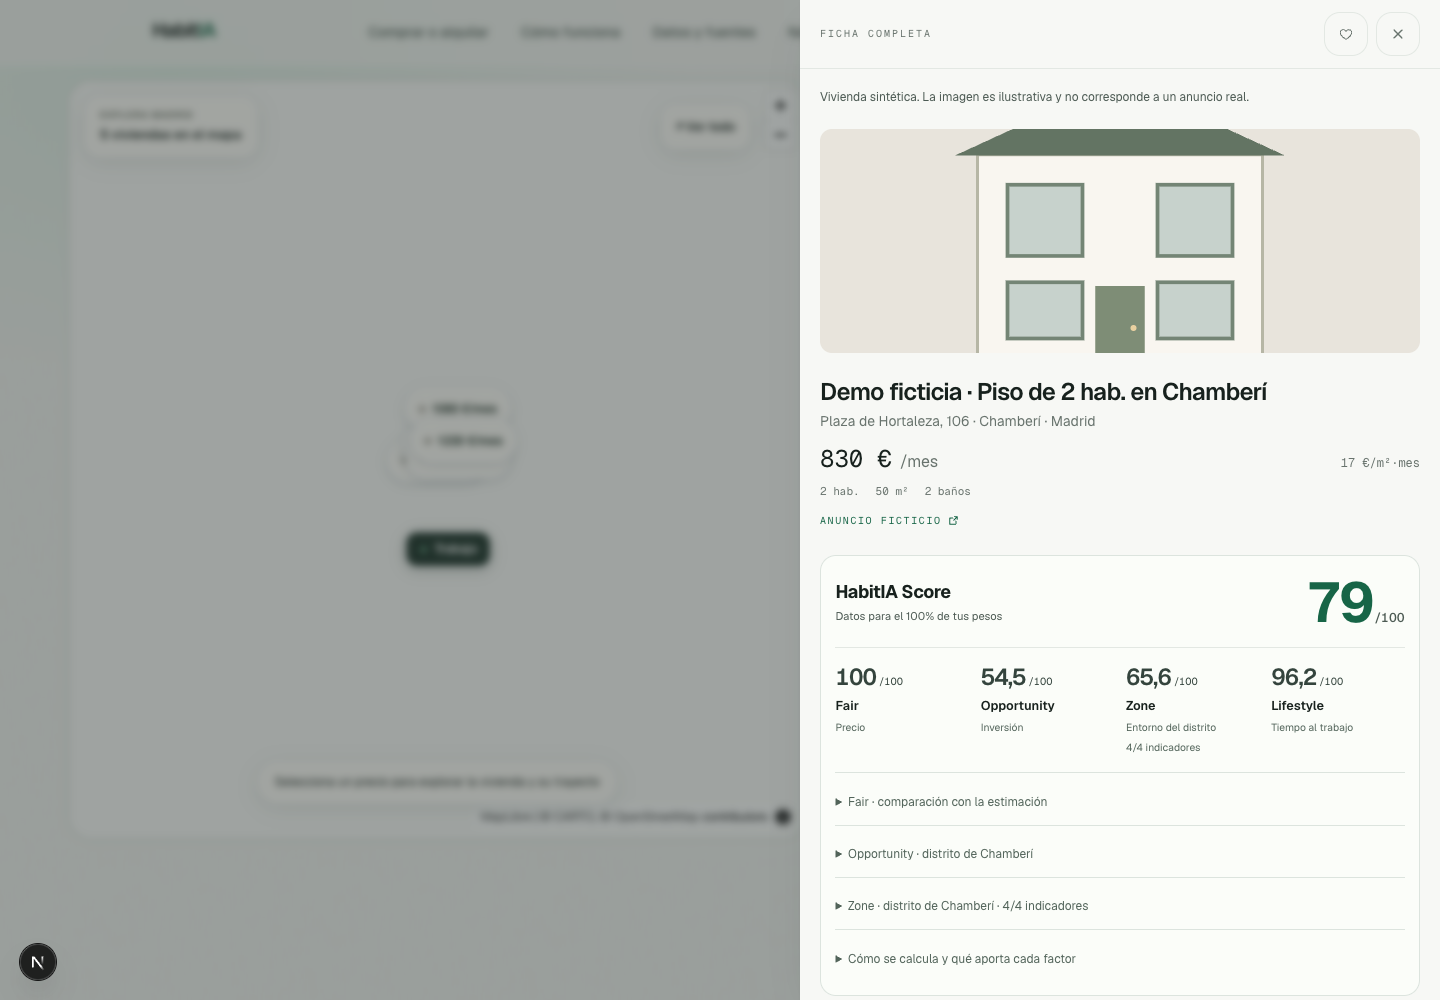
\includegraphics[width=0.9\linewidth]{app_ficha.png}
\caption{Pantalla de inicio (arriba) y ficha de un anuncio sintético de demostración con su puntuación (abajo). Las capturas ilustran la interfaz; no constituyen observaciones del mercado.}
\label{fig:capturas}
\end{figure}

\hfill

Los resultados se presentan como tarjetas sobre un mapa, con acceso a la ficha de cada anuncio (Figura~\ref{fig:capturas}). La ficha de cada vivienda muestra el precio anunciado frente a la referencia, las advertencias asociadas a la estimación (por ejemplo, una planta imputada o una variable fuera de rango) y un enlace al anuncio original en Idealista. La aplicación incluye además una calculadora que compara la compra y el alquiler con supuestos editables; sus resultados son independientes del modelo de precios y se presentan como tales.

% ============================= 8 =============================
\clearpage
\section{Conclusiones y trabajo futuro}

Este trabajo ha desarrollado HabitIA, una herramienta que combina un modelo de estimación de precios de vivienda con una aplicación de búsqueda y comparación de anuncios en Madrid capital. El modelo se construyó a partir de 75.469 viviendas anunciadas en 2018, enriquecidas con indicadores municipales de barrio, mediante un proceso que separó entrenamiento y prueba para el modelado y documentó las decisiones sobre las variables, con la limitación de una exploración inicial del conjunto completo. Entre las familias comparadas, XGBoost obtuvo los mejores resultados. En su versión aplicable a anuncios actuales, alcanza un error porcentual mediano del 9,3 \% en el conjunto de prueba, con cuatro de cada cinco viviendas estimadas dentro de un margen del 20 \%.

Tres resultados merecen destacarse. En primer lugar, el precio depende sobre todo de la superficie y de la localización, y unas pocas variables explican casi toda la variación. En segundo lugar, renunciar a la información catastral para poder usar el modelo en producción tiene un coste real pero limitado, de alrededor de un punto de error mediano, concentrado en las viviendas pequeñas y baratas. Por último, el análisis ha mostrado la importancia de interpretar con cuidado las relaciones aparentes, como la de la tasa de incidencias con el precio, que resultó reflejar la centralidad de los barrios.

\subsection{Limitaciones}

La principal limitación es temporal. El modelo aprende precios anunciados de 2018, no precios de cierre, y su traslado a 2026 depende de índices de distrito proyectados a partir de series que terminan en 2025 (venta) y 2024 (alquiler). Esta actualización supone que la estructura relativa de precios dentro de cada distrito y la distancia entre precio anunciado y precio de cierre se han mantenido estables. El indicador de incidencias procede de 2026, mientras que el índice de vulnerabilidad corresponde a 2018, el mismo año que los anuncios.

El modelo tampoco dispone de información sobre el estado de conservación, las vistas o la condición de ático, y en producción depende de lo que el anunciante escriba en la descripción para conocer siete equipamientos. La renta mensual es una derivación a partir de ratios de distrito que no se ha validado de forma independiente, y el modelo no es monótono respecto a la superficie, por lo que no sirve para simular reformas. En la aplicación, las escalas del HabitIA Score son provisionales, y los componentes Opportunity y Zone, calculados por distrito, discriminan poco entre viviendas cercanas. Tampoco se ha evaluado de forma sistemática el comportamiento del asistente conversacional.

\subsection{Trabajo futuro}

El siguiente paso natural es evaluar el sistema con datos actuales: una muestra de anuncios recientes, idealmente con precios de cierre, permitiría medir la precisión real en 2026 por distrito, tipología y calidad de la información, y sustituir la proyección de los índices por el dato registral en cuanto se publique. Esa misma muestra permitiría entrenar un modelo específico de alquiler y calibrar intervalos de predicción, por ejemplo mediante regresión cuantílica o predicción conformal, que sustituyan la escala provisional del componente Fair. También sería conveniente validar el modelo con particiones espaciales o temporales, ya que los indicadores de barrio pueden verse favorecidos por la partición aleatoria utilizada.

% ============================= 14 =============================
\clearpage
\section{Bibliografía}

\begin{enumerate}[label={[\arabic*]},leftmargin=2.2em,itemsep=6pt]
\item Rey-Blanco, D., Arbués, P., López, F. A. y Páez, A. (2024). A geo-referenced micro-data set of real estate listings for Spain's three largest cities. \emph{Environment and Planning B: Urban Analytics and City Science}. Paquete R \emph{idealista18}: \url{https://github.com/paezha/idealista18}
\item Chen, T. y Guestrin, C. (2016). XGBoost: A Scalable Tree Boosting System. \emph{Proceedings of KDD}, 785--794. \url{https://doi.org/10.1145/2939672.2939785}
\item XGBoost Developers. \emph{XGBoost Parameters}. \url{https://xgboost.readthedocs.io/en/stable/parameter.html}
\item Duan, N. (1983). Smearing Estimate: A Nonparametric Retransformation Method. \emph{Journal of the American Statistical Association}, 78(383), 605--610. \url{https://doi.org/10.2307/2288126}
\item XGBoost Developers. \emph{Python API Reference} e \emph{Introduction to Model IO}. \url{https://xgboost.readthedocs.io/en/stable/python/python_api.html} y \url{https://xgboost.readthedocs.io/en/stable/tutorials/saving_model.html}
\item Perales Lara, T. (2026). \emph{HabitIA Predictor}. Documentación técnica de la generación del modelo de predicción de precios del proyecto HabitIA \url{https://github.com/tomasper17/house-pricing-model-habitia}.
\item Equipo HabitIA (2026). \emph{Verificación del modelo XGBoost y de su integración}. Código del proyecto, informes de verificación y anexos de esta memoria.
\item Ayuntamiento de Madrid. \emph{Sistema estatal de índices de referencia del precio del alquiler de viviendas (SERPAVI): resultados por sección censal}. Portal de estadística municipal.
\item Instituto Nacional de Estadística. \emph{Cartografía digitalizada de secciones censales a 1 de enero de 2018}. \url{https://www.ine.es}
\item Ayuntamiento de Madrid. \emph{Incidencias recibidas en la emisora central de Policía Municipal} y \emph{Población por distrito y barrio}. \url{https://datos.madrid.es}
\item Ayuntamiento de Madrid. \emph{Índice de vulnerabilidad territorial de barrios y distritos}. \url{https://datos.madrid.es/dataset/300301-0-ranking-vulnerabilidad}
\item Lundberg, S. M., Erion, G., Chen, H., DeGrave, A., Prutkin, J. M., Nair, B., Katz, R., Himmelfarb, J., Bansal, N. y Lee, S.-I. (2020). From local explanations to global understanding with explainable AI for trees. \emph{Nature Machine Intelligence}, 2, 56--67. \url{https://doi.org/10.1038/s42256-019-0138-9}
\item Breiman, L. (2001). Random Forests. \emph{Machine Learning}, 45, 5--32. \url{https://doi.org/10.1023/A:1010933404324}
\end{enumerate}
% ===================== PORTADA (ANEXOS) =====================
\clearpage
\newcounter{paginaanexos}
\setcounter{paginaanexos}{\value{page}}
\begin{titlepage}
\setcounter{page}{\value{paginaanexos}}
\phantomsection
\addcontentsline{toc}{section}{Anexos}
\thispagestyle{empty}
\centering
\vspace*{1.2cm}
{\Large UNIVERSIDAD COMPLUTENSE DE MADRID\par}
\vspace{0.4cm}
{\Large FACULTAD DE ESTUDIOS ESTADÍSTICOS\par}
\vspace{1.6cm}
{\large Máster big data, data science \&\par}
\vspace{0.2cm}
{\large inteligencia artificial 2025-2026\par}
\vspace{0.4cm}
{\large (clase 2)\par}
\vspace{1.6cm}

{\large Trabajo Fin de Máster: HabitIA\par}
\vspace{0.4cm}
{\large Anexos\par}
\vspace{0.7cm}
{\large Equipo:\par}
\vspace{0.3cm}
{\large Mauricio Peón García\par}
{\large João Paulo Nogueira Cunha\par}
{\large Manuel Macedo Púlido\par}
{\large Aldo Mauricio Ress Vilet\par}
{\large Tomás Perales Lara\par}
\vspace{1.4cm}
{\small Madrid \textperiodcentered{} Curso 2025--2026\par}
\end{titlepage}

% ===================== ÍNDICE DE ANEXOS =====================
\setcounter{page}{\value{paginaanexos}}
\stepcounter{page}
\clearpage
{\Large\sffamily\bfseries Índice de anexos\par}\vspace{1em}
\newcommand{\anxentry}[2]{\noindent #1\hspace{0.6em}#2\dotfill \pageref{anx:#1}\par\vspace{2pt}}
\anxentry{1}{Artefactos de inferencia}
\anxentry{2}{Diccionario de entradas físicas}
\anxentry{3}{Diccionario territorial y rangos}
\anxentry{4}{Configuración e importancia}
\anxentry{5}{Construcción de las tablas territoriales}
\anxentry{6}{Índices de distrito}
\anxentry{7}{Métricas y alcance de evaluación}
\anxentry{8}{Transformaciones de texto}
\anxentry{9}{Ejemplo de respuesta}
\anxentry{10}{Casos de validación}
\anxentry{11}{Sensibilidad del modelo}
\anxentry{12}{Ejecución y verificación}
\anxentry{13}{Reproducción experimental y trazabilidad}
\anxentry{14}{Detalle técnico de la aplicación}

% ---- Composición compacta de los anexos técnicos ----
\small
\setlength{\parskip}{0.5em}
\renewcommand{\arraystretch}{1.15}

% ===================== ANEXO 1 =====================
\clearpage\refstepcounter{anexo}\phantomsection\label{anx:\theanexo}%
\pdfbookmark[1]{Anexo \theanexo}{anexo.\theanexo}
\section*{\theanexo\hspace{0.6em}Artefactos de inferencia}

La inferencia utiliza un XGBoost y cinco archivos de metadatos y datos territoriales. Identificador: \texttt{habitIA-xgboost-2018-v3}; paquete 3; API HTTP 3.3.0. Los pesos se entrenaron con los precios de 2018, y las tablas territoriales proyectan la venta, la renta y el alquiler de barrio a 2026.

\begin{center}
\begin{tabularx}{\linewidth}{@{}l r L@{}}
\toprule
\thead{Archivo} & \thead{Tamaño en bytes} & \thead{Contenido} \\
\midrule
barrios.parquet & 334334 & 131 geometrías \\
indices\_distrito.parquet & 10357 & 21 distritos \\
metadatos.json & 4120 & 21 entradas y configuración \\
modelo.json & 30194740 & 410 árboles \\
pois.parquet & 9422 & 396 puntos \\
variables\_barrio.parquet & 12310 & 131 barrios \\
\bottomrule
\end{tabularx}
\end{center}

\refstepcounter{anexosub}\needspace{3\baselineskip}%
\subsection*{\theanexo\hspace{0.3em}\arabic{anexosub}\hspace{0.45em}Huellas de los artefactos}

\noindent{\ttfamily\footnotesize
barrios.parquet\\
4a6fa529722ec3f4aa0bae6b652e85e9de226806354bc708674b9c58812fa729\\[4pt]
indices\_distrito.parquet\\
12be67eb7f19f3d0327521ae8ea1065b3ed661e166cf3aaa8bd5f324a2acead4\\[4pt]
metadatos.json\\
ff21768f6dd322b244b028b9ad0621f386e2b3dec817a0b2b68f4f25c38cb1ee\\[4pt]
modelo.json\\
e5526aca6001741f24eb976dbd9607df131b3822b5b5a01b66c6c92af2a9d748\\[4pt]
pois.parquet\\
ef99f3e59ee22ebec4d0e7b8154010ad60cf8c48891686c1799f675af8033322\\[4pt]
variables\_barrio.parquet\\
2ef587ae1e3c121f38503ac68fe06d224972240b75faa2c13998cf0eef62c337\par}

\vspace{0.8em}
El manifiesto \texttt{servicio/manifiesto\_v3.json} contiene las huellas SHA-256 que el instalador y el servicio comprueban para identificar los artefactos. El código de inferencia se encuentra en \texttt{predictor\_v3/}. Esta separación permite distribuir los pesos sin incorporarlos al historial de Git y verificar que la aplicación utiliza la versión documentada.

Estos artefactos son el resultado final del proceso de modelado documentado en el repositorio del modelo [6]. El conjunto de trabajo \texttt{data/interim/habitia\_madrid\_2018.csv} (75.469 viviendas y 43 columnas) se construye en el cuaderno 00; la partición de entrenamiento y prueba y las matrices de cada variante, en el cuaderno 04; y el modelo exportado procede del cuaderno 07 mediante \texttt{python -m src.predictor exportar}. El anexo 13 describe cómo reproducir el proceso completo, y el anexo 12, cómo ejecutar únicamente la inferencia a partir de estos artefactos.

% ===================== ANEXO 2 =====================
\clearpage\refstepcounter{anexo}\phantomsection\label{anx:\theanexo}%
\pdfbookmark[1]{Anexo \theanexo}{anexo.\theanexo}
\section*{\theanexo\hspace{0.6em}Diccionario de entradas físicas}

El orden de esta tabla y de la siguiente coincide con el almacenado en el modelo. Los booleanos se convierten en 0 o 1 después de validar los tipos de entrada. ``Sin mención'' y ``sin descripción'' producen 0 en los atributos extraídos del texto; no constituyen una medición de ausencia real del equipamiento.

\begin{center}
\begin{tabularx}{\linewidth}{@{}c >{\scriptsize}l >{\scriptsize\RaggedRight\arraybackslash}p{3.5cm} L@{}}
\toprule
\thead{N} & \thead{Variable} & \thead{Origen en el anuncio} & \thead{Transformación} \\
\midrule
1 & CONSTRUCTEDAREA & size & m²; obligatorio y positivo \\
2 & ROOMNUMBER & rooms & Entero observado no negativo \\
3 & BATHNUMBER & bathrooms & Entero observado no negativo \\
4 & HASTERRACE & description & Terraza; reglas de mención y negación \\
5 & HASLIFT & hasLift; después description & Ascensor; prevalece el campo estructurado \\
6 & HASAIRCONDITIONING & description & Aire acondicionado; excluye preinstalación \\
7 & HASPARKINGSPACE & parkingSpace.\allowbreak hasParkingSpace & Garaje; campo ausente equivale a 0 \\
8 & HASBOXROOM & description & Trastero; reglas de inclusión \\
9 & HASWARDROBE & description & Armarios empotrados \\
10 & HASSWIMMINGPOOL & description & Piscina; distingue menciones al entorno \\
11 & HASDOORMAN & description & Portero o conserje; excluye portero automático \\
12 & HASGARDEN & description & Jardín; descarta referencias a parques próximos \\
13 & ISDUPLEX & propertyType o detailedType.subTypology & Indicador de dúplex \\
14 & ISSTUDIO & propertyType o detailedType.subTypology & Indicador de estudio \\
15 & FLOORCLEAN & floor & Planta numérica; imputación con 2 si no se interpreta \\
\bottomrule
\end{tabularx}
\end{center}

El campo de planta se recibe como texto. Los códigos \texttt{bj} y \texttt{en} se convierten en 0; \texttt{ss} y \texttt{st}, en −1. Un texto no interpretable o una planta ausente se sustituye por la mediana registrada. Las coordenadas y el precio anunciado son contexto de construcción: las primeras permiten obtener distancias y barrio; el segundo solo interviene al comparar la estimación con la oferta.

El modelo no tiene entrada propia de conservación, parcela, vistas, antigüedad o ático. El predictor sí usa reglas sobre la descripción para abstenerse ante \texttt{a\_reformar} y \texttt{ocupada}, incluida vivienda alquilada, en compra y alquiler. La marca estructurada \texttt{newDevelopment} añade \texttt{obra\_nueva} a calidad sin bloquear la predicción. Estas reglas delimitan el dominio; no modelan el estado ni comprenden el texto de forma general.
% ===================== ANEXO 3 =====================
\clearpage\refstepcounter{anexo}\phantomsection\label{anx:\theanexo}%
\pdfbookmark[1]{Anexo \theanexo}{anexo.\theanexo}
\section*{\theanexo\hspace{0.6em}Diccionario territorial y rangos}

\begin{center}
\begin{tabularx}{\linewidth}{@{}c l L@{}}
\toprule
\thead{N} & \thead{Variable} & \thead{Definición operativa} \\
\midrule
16 & DISTANCE\_TO\_CITY\_CENTER & Haversine al único punto City\_Center, en km \\
17 & DISTANCE\_TO\_METRO & Mínima haversine a 240 puntos de metro, en km \\
18 & DISTANCE\_TO\_CASTELLANA & Mínima haversine a 155 puntos del eje, en km \\
19 & alq\_mediana\_eur\_m2\_barrio & Agregado ponderado de medianas de alquiler transformado a la escala del entrenamiento \\
20 & delitos\_per\_10k\_barrio & Indicador territorial de incidencias por 10.000 habitantes \\
21 & indice\_vulnerabilidad & Valor territorial de vulnerabilidad incluido en la tabla \\
\bottomrule
\end{tabularx}
\end{center}

\refstepcounter{anexosub}\needspace{3\baselineskip}%
\subsection*{\theanexo\hspace{0.3em}\arabic{anexosub}\hspace{0.45em}Rangos registrados de entrenamiento}

\begin{center}
\begin{tabularx}{\linewidth}{@{}L r r@{}}
\toprule
\thead{Variable} & \thead{Mínimo} & \thead{Máximo} \\
\midrule
CONSTRUCTEDAREA & 21,000 & 985,000 \\
ROOMNUMBER & 0,000 & 93,000 \\
BATHNUMBER & 0,000 & 20,000 \\
FLOORCLEAN & −1,000 & 11,000 \\
DISTANCE\_TO\_CITY\_CENTER & 0,008 & 14,159 \\
DISTANCE\_TO\_METRO & 0,001 & 9,374 \\
DISTANCE\_TO\_CASTELLANA & 0,001 & 12,574 \\
alq\_mediana\_eur\_m2\_barrio & 6,707 & 14,839 \\
delitos\_per\_10k\_barrio & 25,440 & 1.395,230 \\
indice\_vulnerabilidad & 0,005400 & 0,012100 \\
Nueve equipamientos y dos tipos & 0 & 1 \\
\bottomrule
\end{tabularx}
\end{center}

Estos mínimos y máximos se leen del metadato; no son límites de validación de negocio. El servicio exige superficie positiva y rechaza valores superiores a 367 m². Una superficie de 20 m² queda por debajo del mínimo entrenado de 21 m² y produce advertencia. Los campos de habitaciones y baños carecen de un máximo de plausibilidad en la validación actual de la API: un valor superior al rango se advierte, pero puede seguir produciendo una predicción.

Una geometría válida no garantiza apoyo en entrenamiento. Los barrios 041, 046 y 096 superan el rango de alquiler y el 194 queda bajo el mínimo de incidencias; vulnerabilidad respeta su rango. La política de abstención debe considerar cobertura, plausibilidad y apoyo real. Los avisos informan de rangos; \texttt{a\_reformar} y \texttt{ocupada} impiden valorar.

% ===================== ANEXO 4 =====================
\clearpage\refstepcounter{anexo}\phantomsection\label{anx:\theanexo}%
\pdfbookmark[1]{Anexo \theanexo}{anexo.\theanexo}
\section*{\theanexo\hspace{0.6em}Configuración e importancia}

El JSON confirma objetivo \texttt{reg:squarederror}, 21 entradas, 410 árboles, 542.414 nodos y 271.412 hojas. Todos los árboles alcanzan profundidad 12. Las siguientes importancias proceden de sumar \texttt{loss\_changes} en las divisiones por variable y normalizar la suma total; la frecuencia cuenta esas divisiones. Las hojas no se cuentan como divisiones.

\begin{center}
\begin{tabularx}{\linewidth}{@{}L r r@{}}
\toprule
\thead{Variable} & \thead{Divisiones} & \thead{Ganancia total normalizada} \\
\midrule
CONSTRUCTEDAREA & 34.128 & 50,36 \% \\
alq\_mediana\_eur\_m2\_barrio & 17.821 & 16,18 \% \\
indice\_vulnerabilidad & 13.636 & 11,28 \% \\
BATHNUMBER & 5.858 & 5,42 \% \\
HASLIFT & 4.161 & 2,80 \% \\
DISTANCE\_TO\_CASTELLANA & 36.316 & 2,36 \% \\
DISTANCE\_TO\_CITY\_CENTER & 36.778 & 1,96 \% \\
delitos\_per\_10k\_barrio & 17.977 & 1,59 \% \\
FLOORCLEAN & 20.667 & 1,50 \% \\
ROOMNUMBER & 10.707 & 1,43 \% \\
DISTANCE\_TO\_METRO & 35.291 & 1,02 \% \\
HASBOXROOM & 4.334 & 0,95 \% \\
HASGARDEN & 3.150 & 0,55 \% \\
HASSWIMMINGPOOL & 2.044 & 0,49 \% \\
HASDOORMAN & 4.242 & 0,44 \% \\
HASPARKINGSPACE & 3.395 & 0,38 \% \\
HASTERRACE & 6.022 & 0,34 \% \\
HASWARDROBE & 6.545 & 0,33 \% \\
HASAIRCONDITIONING & 6.321 & 0,33 \% \\
ISSTUDIO & 629 & 0,23 \% \\
ISDUPLEX & 980 & 0,06 \% \\
\bottomrule
\end{tabularx}
\fuente{Fuente: elaboración propia a partir de modelo.json. La ganancia se calcula sumando loss\_changes en las divisiones de cada variable.}
\end{center}

Parámetros completos registrados:
\begin{lstlisting}
n_estimators=410; max_depth=12
learning_rate=0.08788507761298064
subsample=0.9568742693092576
colsample_bytree=0.528081635815584
min_child_weight=5; gamma=0.0005361223891082169
reg_alpha=0.0034879036214009018
reg_lambda=8.659692055247017
\end{lstlisting}

Estos valores proceden de la búsqueda de hiperparámetros del cuaderno 06 (capítulo~\ref{sec:metodologia}): una búsqueda aleatoria en dos etapas con validación cruzada de cinco particiones sobre la variante desplegable, seguida de parada temprana en cada partición. Las iteraciones óptimas por partición fueron 398, 412, 411, 410 y 388, y su mediana fija el número de árboles en 410. La configuración elegida queda registrada en \texttt{data/results/modelos\_seleccionados\_06.json}, que el cuaderno 07 lee para reentrenar el modelo sobre todo el conjunto de entrenamiento.

La frecuencia de uso de una variable no determina su aportación a la función objetivo: la distancia al centro interviene en más divisiones que la superficie, pero con una ganancia acumulada mucho menor. La ganancia tampoco expresa euros ni la dirección del efecto; para eso, el capítulo~\ref{sec:resultados} utiliza valores SHAP, que ofrecen una lectura más directa y coinciden con esta tabla en las tres variables principales. La interfaz web resume la ganancia media por división, una magnitud distinta de la ganancia total utilizada aquí.

% ===================== ANEXO 5 =====================
\clearpage\refstepcounter{anexo}\phantomsection\label{anx:\theanexo}%
\pdfbookmark[1]{Anexo \theanexo}{anexo.\theanexo}
\section*{\theanexo\hspace{0.6em}Construcción de las tablas territoriales}

\refstepcounter{anexosub}\needspace{3\baselineskip}%
\subsection*{\theanexo\hspace{0.3em}\arabic{anexosub}\hspace{0.45em}Geometría y puntos de interés}

Las geometrías proceden del seccionado censal de 2018, filtrado por el código municipal 28079, proyectado a EPSG 25830 y agregado por barrio con el mapeo de 2026. El artefacto contiene 131 geometrías válidas y no vacías, sin códigos duplicados. La asignación comprueba primero la contención estricta del punto. Si falla, utiliza el barrio más próximo hasta 500 m y activa la advertencia \texttt{barrio\_rescatado}.

La tabla de puntos contiene 396 registros sin nulos: uno central, 240 de metro y 155 de Castellana. La fórmula haversine emplea un radio terrestre de 6.371,0088 km. Se selecciona la distancia mínima entre el anuncio y los puntos de cada tipo. No se utilizan redes viarias, horarios de transporte ni una proyección continua sobre la línea de Castellana.

\refstepcounter{anexosub}\needspace{3\baselineskip}%
\subsection*{\theanexo\hspace{0.3em}\arabic{anexosub}\hspace{0.45em}Alquiler de barrio}

El alquiler de barrio agrega medianas por sección, ponderadas por viviendas. El último dato es de 2024; barrio y ciudad se proyectan a 2026 según su tendencia log-lineal desde 2018. Después se calcula \texttt{alquiler\_2026\_crudo / 1,3642729473419677 × 0,9285634138823831}. El primer factor deflacta a 2018; el segundo calibra el método con la mediana de cocientes entre el valor entrenado y el agregado de 2018 en barrios comunes.

Los atributos registran agregados urbanos de 11,3966145470 en 2018 y 15,5480929178 proyectado a 2026. La transformación coincide con la columna usada en los 131 barrios, con diferencia máxima 0. Un barrio con menos de dos años de datos toma la tendencia urbana. La serie por sección censal (\texttt{data/raw/madrid\_alquiler/}), la agregación, la proyección y la calibración están implementadas en \texttt{src/produccion.py} y \texttt{src/indices\_precio.py}, y el cuaderno 08 (apartado 2.3) las documenta paso a paso.

\refstepcounter{anexosub}\needspace{3\baselineskip}%
\subsection*{\theanexo\hspace{0.3em}\arabic{anexosub}\hspace{0.45em}Procedencia y excepciones observadas}

\begin{center}
\begin{tabularx}{\linewidth}{@{}L L@{}}
\toprule
\thead{Componente} & \thead{Resultado de inspección} \\
\midrule
Incidencias y vulnerabilidad & 130 barrios con los valores de entrenamiento; el 194 calculado desde las fuentes \\
Alquiler fuera de rango & Barrios 041, 046 y 096 por encima del máximo entrenado \\
Incidencias fuera de rango & Barrio 194 por debajo del mínimo entrenado \\
Vulnerabilidad & Ningún valor fuera del rango registrado \\
Completitud & Sin nulos en las columnas publicadas de la tabla \\
\bottomrule
\end{tabularx}
\end{center}

Los indicadores de incidencias y vulnerabilidad se construyen en el cuaderno 00 a partir de las fuentes municipales: las incidencias de la Policía Municipal de 2026 y la población por barrio del mismo año (\texttt{src/crime\_indices.py} y \texttt{src/aux\_functions.py}), y la edición de 2018 del índice de vulnerabilidad, contenida en el fichero \texttt{vulnerabilidad\_barrios\_2020.csv} (\texttt{src/vulnerability\_indices.py}). En producción se reutilizan los valores de entrenamiento de los 130 barrios con anuncios en 2018; el barrio 194 (El Cañaveral), sin anuncios en el conjunto de trabajo, se calcula directamente desde las mismas fuentes. Como se indica en el capítulo~3, la estadística de incidencias no existe para 2018, de modo que su uso supone que la distribución relativa entre barrios se ha mantenido estable.

% ===================== ANEXO 6 =====================
\clearpage\refstepcounter{anexo}\phantomsection\label{anx:\theanexo}%
\pdfbookmark[1]{Anexo \theanexo}{anexo.\theanexo}
\section*{\theanexo\hspace{0.6em}Índices de distrito}

Factores aplicados, redondeados para lectura; la inferencia conserva la precisión del parquet. $I_d = \text{venta}_{2026} / \text{venta}_{2018}$; $q_d = \text{alquiler}_{2026} / \text{venta}_{2026}$, en mes\textsuperscript{-1}. Los 21 cocientes coinciden con las columnas publicadas. Los niveles de 2026 son proyecciones: los atributos registran venta observada hasta 2025, alquiler hasta 2024 e inicio de tendencia en 2018.

\begin{center}
\begin{tabularx}{\linewidth}{@{}c L r r@{}}
\toprule
\thead{Código} & \thead{Distrito} & \thead{$I_d$ de venta} & \thead{$q_d$ mensual} \\
\midrule
01 & Centro & 1,558746 & 0,00252640 \\
02 & Arganzuela & 1,756827 & 0,00264321 \\
03 & Retiro & 1,792965 & 0,00216517 \\
04 & Salamanca & 1,876612 & 0,00195128 \\
05 & Chamartín & 1,670072 & 0,00233849 \\
06 & Tetuán & 1,749759 & 0,00297842 \\
07 & Chamberí & 1,685388 & 0,00227874 \\
08 & Fuencarral-El Pardo & 1,742970 & 0,00254481 \\
09 & Moncloa-Aravaca & 1,656751 & 0,00267242 \\
10 & Latina & 1,784942 & 0,00333830 \\
11 & Carabanchel & 1,798154 & 0,00359251 \\
12 & Usera & 2,116378 & 0,00332761 \\
13 & Puente de Vallecas & 1,920223 & 0,00396780 \\
14 & Moratalaz & 1,834847 & 0,00297833 \\
15 & Ciudad Lineal & 1,741034 & 0,00287186 \\
16 & Hortaleza & 1,631710 & 0,00270289 \\
17 & Villaverde & 1,876226 & 0,00397004 \\
18 & Villa de Vallecas & 1,618235 & 0,00366366 \\
19 & Vicálvaro & 2,258196 & 0,00280126 \\
20 & San Blas-Canillejas & 1,614348 & 0,00372369 \\
21 & Barajas & 1,475936 & 0,00288879 \\
\bottomrule
\end{tabularx}
\end{center}

La renta aplica el ratio mensual proyectado a 2026 a la venta del mismo año. No incluye vacancia, gastos, impuestos, financiación ni conservación. Los indicadores derivados de estos ratios son resultados aritméticos, no rendimientos observados. Las tasas anuales de crecimiento acompañan los niveles proyectados, pero no son nuevas entradas del XGBoost.

Los índices se construyen en \texttt{src/indices\_precio.py} a partir de dos series del Ayuntamiento de Madrid: el precio medio declarado de compraventa por distrito, de origen registral, para 2007--2025 (\texttt{data/raw/madrid\_compraventa/}), y la renta por sección censal del SERPAVI para 2011--2024 (\texttt{data/raw/madrid\_alquiler/}). Para cada distrito se ajusta una tendencia log-lineal desde 2018 y se proyecta el valor de 2026; la mediana entre distritos equivale a un crecimiento anual del 6,4 \% en venta y del 3,8 \% en alquiler. La ventana comienza en 2018, el año base del modelo, porque incluir los años anteriores a 2014 incorporaría la caída de precios posterior a 2008 y reduciría la tendencia a la mitad. El cuaderno 08 (apartado 3) detalla las fórmulas y los resultados por distrito.
% ===================== ANEXO 7 =====================
\clearpage\refstepcounter{anexo}\phantomsection\label{anx:\theanexo}%
\pdfbookmark[1]{Anexo \theanexo}{anexo.\theanexo}
\section*{\theanexo\hspace{0.6em}Métricas y alcance de evaluación}

Esta tabla define las métricas del modelo de producción que se presentan en el capítulo~\ref{sec:resultados}. Se calculan en el cuaderno 07 sobre las 15.094 viviendas del conjunto de prueba, reservadas para la evaluación del modelado, y quedan registradas en \texttt{metadatos.json}. En las métricas en euros y porcentajes, $y$ es el precio anunciado y $p$ la predicción en euros corregida con el factor de \emph{smearing}. RMSE log y $R^2$ log se calculan sobre la salida logarítmica original del modelo, antes de esa corrección.

\begin{center}
\footnotesize
\begin{tabularx}{\linewidth}{@{}l L r@{}}
\toprule
\thead{Medida} & \thead{Definición de referencia} & \thead{Valor registrado} \\
\midrule
MAE & Media de $|p - y|$ & 49.220,1987 € \\
MdAE & Mediana de $|p - y|$ & 23.708,4844 € \\
MAPE & $100 \times$ media de $(|p - y| / y)$ & 13,6151 \% \\
MdAPE & $100 \times$ mediana de $(|p - y| / y)$ & 9,2990 \% \\
Dentro de ±10 \% & Proporción con $|p - y| / y \le 0{,}10$ & 52,7561 \% \\
Dentro de ±20 \% & Proporción con $|p - y| / y \le 0{,}20$ & 80,5552 \% \\
RMSE log & Raíz de la media del error logarítmico al cuadrado & 0,1856103494 \\
R² log & 1 menos la razón entre error cuadrático y variación total en logaritmos & 0,9398942152 \\
Sesgo mediano porcentual & $100 \times$ (mediana de $p / y$ $-$ 1); positivo indica sobrestimación & 1,0254336376 \% \\
RMSE log de validación cruzada & Media de las cinco particiones sobre el conjunto de entrenamiento (cuaderno 06) & 0,1857717187 \\
\bottomrule
\end{tabularx}
\end{center}

\refstepcounter{anexosub}\needspace{3\baselineskip}%
\subsection*{\theanexo\hspace{0.3em}\arabic{anexosub}\hspace{0.45em}Protocolo de evaluación}

La partición se realizó en el cuaderno 04 de forma aleatoria (80/20, semilla 42) sobre el conjunto de trabajo, que contiene un único registro por inmueble; por construcción, ninguna vivienda aparece a la vez en entrenamiento y prueba. Los valores de imputación, los cortes de las variables discretizadas y los parámetros de estandarización se ajustaron solo con el conjunto de entrenamiento. La selección de variables (cuaderno 03) evaluó la contribución al ajuste y el BIC sobre entrenamiento. La comparación de familias (cuaderno 05) y la búsqueda de hiperparámetros (cuaderno 06) utilizaron validación cruzada de cinco particiones dentro del entrenamiento; el cuaderno 07 evaluó los modelos finales en prueba. Los cuadernos 01 y 02 habían explorado previamente el conjunto completo, por lo que la prueba no fue ajena a todas las decisiones sobre transformaciones. El factor de \emph{smearing} se estimó con residuos fuera de muestra de una validación cruzada sobre el entrenamiento, sin utilizar el conjunto de prueba.

El cuaderno 07 complementa las métricas agregadas con un análisis de incertidumbre y de errores por segmento: intervalos de confianza \emph{bootstrap} del RMSE log (IC95 [0,1811; 0,1906] para el modelo de producción), una comparación pareada con el modelo que utiliza variables catastrales y la desagregación del error por decil de precio, distrito y tamaño. Los principales resultados se resumen en el capítulo~\ref{sec:resultados}.

La evaluación tiene tres límites. Mide el error frente a precios anunciados de 2018, no frente a precios actuales ni de cierre. La partición aleatoria puede favorecer a los indicadores de barrio frente a una partición espacial o temporal, y la exploración inicial del conjunto completo limita su independencia. Y no incluye una evaluación específica de la renta mensual ni intervalos de predicción calibrados; el 19,4 \% de viviendas con error superior al 20 \% describe el conjunto de prueba, no la probabilidad de error de una vivienda concreta.

\refstepcounter{anexosub}\needspace{3\baselineskip}%
\subsection*{\theanexo\hspace{0.3em}\arabic{anexosub}\hspace{0.45em}Comprobación de exportación}

Al exportar el modelo al formato nativo de XGBoost, se comparan sus predicciones logarítmicas sobre el conjunto de prueba con las del modelo original, con una tolerancia de $10^{-5}$; la diferencia registrada es 0,0. La integración con la aplicación se verificó por separado con 131 anuncios sintéticos por barrio y 21 casos límite (anexo~14).

% ===================== ANEXO 8 =====================
\clearpage\refstepcounter{anexo}\phantomsection\label{anx:\theanexo}%
\pdfbookmark[1]{Anexo \theanexo}{anexo.\theanexo}
\section*{\theanexo\hspace{0.6em}Transformaciones de texto}

El extractor normaliza mayúsculas, tildes y espacios y aplica patrones de texto con ventanas de contexto. Registra mención, negación y falta de texto. Cuando hay una afirmación y una negación reconocidas para el mismo atributo, la regla puede conservar la afirmación y marcar conflicto. El predictor final consume el indicador binario; las marcas detalladas de conflicto no forman parte de su respuesta de calidad.

\begin{center}
\begin{tabularx}{\linewidth}{@{}L L L@{}}
\toprule
\thead{Caso sintético} & \thead{Entrada relevante} & \thead{Resultado observado} \\
\midrule
Terraza afirmada & Piso con terraza & HASTERRACE = 1 \\
Terraza negada & Piso sin terraza & HASTERRACE = 0 \\
Piscina del entorno & Cerca de la piscina municipal & HASSWIMMINGPOOL = 0 \\
Portero electrónico & Portero automático & HASDOORMAN = 0 \\
Preinstalación & Preinstalación de aire acondicionado & HASAIRCONDITIONING = 0 \\
Afirmación y negación & Negación y afirmación separadas por texto & HASTERRACE = 1 \\
Ascensor estructurado negativo & hasLift=false; texto con ascensor & HASLIFT = 0 \\
Ascensor solo en texto & hasLift ausente; texto con ascensor & HASLIFT = 1 y marca de origen textual \\
Texto contradice la API & hasLift=true; texto sin ascensor & HASLIFT = 1 \\
Garaje solo en texto & Campo de garaje ausente; texto afirmativo & HASPARKINGSPACE = 0 \\
Descripción ausente & description sin valor & Siete atributos textuales a 0 y sin\_descripcion \\
\bottomrule
\end{tabularx}
\fuente{Fuente: elaboración propia mediante 12 casos sintéticos de extracción de atributos. La tabla agrupa los comportamientos observados; los restantes campos mantienen los valores del caso base.}
\end{center}

La prioridad del campo estructurado se mantiene aunque el texto lo contradiga. Esto permite transformar las mismas entradas de forma reproducible, pero no resuelve cuál de las fuentes describe correctamente el inmueble. Un garaje mencionado únicamente en la descripción no llega al modelo. En ausencia de texto, los equipamientos no inferibles dejan de estar presentes en la matriz.

La verificación de patrones sintéticos confirma ejemplos concretos de la implementación y no calcula precisión lingüística. Para medir falsos positivos y negativos se necesita una muestra de anuncios anotada manualmente. Debe incluir textos ambiguos, instalaciones opcionales, equipamiento comunitario, abreviaturas y contradicciones. Si se modifica el tratamiento de ausencias, será necesario comprobar su compatibilidad con los atributos de entrenamiento antes de sustituir la regla vigente.

% ===================== ANEXO 9 =====================
\clearpage\refstepcounter{anexo}\phantomsection\label{anx:\theanexo}%
\pdfbookmark[1]{Anexo \theanexo}{anexo.\theanexo}
\section*{\theanexo\hspace{0.6em}Ejemplo de respuesta}

Ejemplo local con información sintética. La misma vivienda se puede enviar con \texttt{operation=rent} y \texttt{price=1500} para comprobar la comparación mensual. El servicio necesita un token privado configurado en el entorno. El precio del anuncio puede omitirse: la estimación sigue disponible y la brecha queda vacía.

\begin{lstlisting}
{
  "anuncios": [{
    "propertyCode": "caso-sintetico",
    "operation": "sale",
    "municipality": "Madrid",
    "propertyType": "flat",
    "size": 80, "rooms": 2, "bathrooms": 1,
    "latitude": 40.4168, "longitude": -3.7038,
    "floor": "2", "hasLift": true,
    "parkingSpace": {"hasParkingSpace": true},
    "description": "Piso con terraza, aire acondicionado, armarios empotrados y trastero.",
    "price": 450000
  }],
  "renivelar": true,
  "explicar": false
}
\end{lstlisting}

\begin{center}
\begin{tabularx}{\linewidth}{@{}L l l@{}}
\toprule
\thead{Campo de respuesta} & \thead{Compra} & \thead{Alquiler} \\
\midrule
operation & sale & rent \\
precio\_estimado & 506.052,6113 € & 506.052,6113 € \\
precio\_comparacion & 506.052,6113 & 1.278,4929 \\
unidad\_comparacion & EUR & EUR/mes \\
brecha\_pct & −11,0764 & 17,3256 \\
precio\_estimado\_base & 324.653,6875 € & 324.653,6875 € \\
barrio\_code y distrito\_code & 016 y 01 & 016 y 01 \\
intervalo y banda & null & null \\
alquiler\_validado & false & false \\
\bottomrule
\end{tabularx}
\end{center}

La respuesta incluye versión, huellas de modelo y paquete, años, \texttt{ajuste\_proyectado=true} y \texttt{calidad.obra\_nueva}. La comparación usa venta o renta proyectada a 2026. Fair = clamp(50 − 2,5 × brecha \%, 0, 100) sigue siendo provisional, sin recalibración estadística. Una abstención o una versión obsoleta dejan Fair sin dato y reducen la cobertura del HabitIA Score.

Sin autenticación válida, el servicio devuelve HTTP 401; si el token del servicio no está configurado, devuelve HTTP 503; un lote vacío o de más de 24 anuncios, HTTP 422. Cada problema de anuncio aparece en errores con índice, identificador, estado y detalle. \texttt{a\_reformar} y \texttt{ocupada} se traducen a \texttt{fuera\_ambito} en venta y alquiler. \texttt{obra\_nueva} advierte de dependencia entre anuncios de una misma promoción. La aplicación exige la versión 3.3.0 y el hash actual para reutilizar una valoración.

% ===================== ANEXO 10 =====================
\clearpage\refstepcounter{anexo}\phantomsection\label{anx:\theanexo}%
\pdfbookmark[1]{Anexo \theanexo}{anexo.\theanexo}
\section*{\theanexo\hspace{0.6em}Casos de validación}

Se ejecutaron 21 pruebas automatizadas y 152 casos de paridad: 131 anuncios sintéticos por barrio y 21 casos límite. Se recalcularon el caso base y el barrido de superficie de 111 puntos. Se comprueban autenticación, errores, unidades, abstenciones, obra nueva e integridad de instalación, sin medir precisión inmobiliaria. Los 12 casos de extracción de texto del anexo~8 documentan esas reglas.

\begin{center}
\begin{tabularx}{\linewidth}{@{}L L@{}}
\toprule
\thead{Escenario} & \thead{Resultado del servicio} \\
\midrule
Compra y alquiler válidos & Venta y mensualidad en unidades correspondientes \\
Precio duplicado o ausente & Misma estimación; brecha cambia o queda vacía \\
Descripción ausente & Predicción con siete atributos textuales a 0 y advertencia \\
Planta ausente & Imputación con 2 y marca de calidad \\
Coordenadas ausentes & datos\_insuficientes \\
Coordenadas fuera de Madrid & fuera\_ambito \\
Municipio Barcelona & fuera\_ambito \\
Oficina o chalet & fuera\_ambito \\
Más de 367 m²; a reformar; ocupada/alquilada & fuera\_ambito y Fair ausente; aplica en compra y alquiler \\
367 m² y anuncio de obra nueva & 367 m² admitidos; obra\_nueva advierte sin bloquear \\
Superficie de 20 m² & Resultado con aviso de CONSTRUCTEDAREA fuera de rango \\
94 habitaciones & Resultado con aviso de ROOMNUMBER fuera de rango \\
Booleano enviado como texto & datos\_insuficientes \\
Código de anuncio duplicado & Ambas filas devueltas como error \\
\bottomrule
\end{tabularx}
\end{center}

\refstepcounter{anexosub}\needspace{3\baselineskip}%
\subsection*{\theanexo\hspace{0.3em}\arabic{anexosub}\hspace{0.45em}Lectura de los resultados}

Los rechazos por dominio evitan usos que el modelo no representa. En cambio, las advertencias de rango son informativas y no bloquean todas las combinaciones poco plausibles. Esta distinción debe conservarse en documentación e interfaz. Los casos de 20 m² y 94 habitaciones muestran por qué ``respuesta válida'' significa que el servicio pudo calcularla, no que exista una garantía de apoyo estadístico.

Los 152 casos dieron 141 resultados válidos y 11 abstenciones. La matriz de entrada y la salida nativa coincidieron con las del predictor original del repositorio del modelo; la diferencia máxima de serialización fue $5{,}82 \times 10^{-11}$ euros. Se confirmó 2026 como año predeterminado de exportación y carga. La coincidencia se comprobó usando las mismas dependencias de ejecución; otros entornos pueden introducir pequeñas diferencias de precisión numérica.

La comprobación de \texttt{GET /salud} identificó la API 3.3.0, los 410 árboles y la huella del paquete documentado. La base de precios es 2018 y las referencias de venta y renta se proyectan a 2026. El servicio publicado valoró el caso de 80 m² en 506.052,56 euros y 1.278,49 euros/mes; la diferencia respecto al cálculo local es inferior a cinco céntimos y corresponde a la precisión numérica de la ejecución. Cinco casos verificaron la venta, la renta, las abstenciones por reforma y ocupación, y la advertencia por obra nueva.
% ===================== ANEXO 11 =====================
\clearpage\refstepcounter{anexo}\phantomsection\label{anx:\theanexo}%
\pdfbookmark[1]{Anexo \theanexo}{anexo.\theanexo}
\section*{\theanexo\hspace{0.6em}Sensibilidad del modelo}

Se realizó un barrido sobre el caso de referencia cambiando únicamente CONSTRUCTEDAREA entre 40 y 150 m², en incrementos de un metro. Las otras 20 entradas permanecieron constantes, incluidos dos dormitorios, un baño y la ubicación. Se representó el precio base de 2018 para observar el comportamiento de los árboles sin añadir el índice de venta.

El resultado se representa en la Figura~\ref{fig:sensarea} del capítulo~\ref{sec:resultados}.

\begin{center}
\begin{tabularx}{\linewidth}{@{}L L@{}}
\toprule
\thead{Comprobación} & \thead{Resultado} \\
\midrule
Valores de superficie & 111, entre 40 y 150 m² \\
Incrementos consecutivos & 110 \\
Incrementos con descenso de predicción & 39 \\
Mayor descenso absoluto & De 71 a 72 m²: −27.291,469 € de 2018 \\
Predicciones de ese salto & 364.936,1250 → 337.644,6562 € \\
\bottomrule
\end{tabularx}
\end{center}

La curva contiene tramos planos y saltos, coherentes con una función construida mediante particiones de árboles. En esta combinación sintética no es monótona respecto a superficie. No se estima a partir de ello un porcentaje de anuncios afectados ni la precisión del modelo. Algunas combinaciones pueden alejarse de viviendas frecuentes y el conjunto no incorpora una garantía operativa de monotonía.

Retirar la descripción del caso de 80 m² reduce la venta proyectada de 506.052,61 a 425.980,52 euros, un 15,82 \%. Se eliminan terraza, aire acondicionado, armarios y trastero extraídos del texto; se conservan ascensor y garaje estructurados. Es una diferencia propia del caso, no el valor económico de esos equipamientos.

Los resultados aconsejan evitar explicaciones del tipo ``añadir un metro aumenta el valor en una cantidad fija''. Para evaluar estabilidad se propone repetir estos contrastes sobre anuncios reales, restringiendo las combinaciones a casos plausibles, y comparar predicciones antes y después de cualquier cambio en el tratamiento de atributos ausentes.

% ===================== ANEXO 12 =====================
\clearpage\refstepcounter{anexo}\phantomsection\label{anx:\theanexo}%
\pdfbookmark[1]{Anexo \theanexo}{anexo.\theanexo}
\section*{\theanexo\hspace{0.6em}Ejecución y verificación}

La ejecución local del servicio de inferencia utiliza el repositorio \texttt{habitia-tfm}, el ZIP instalable \texttt{habitia-modelo-v3.3.zip} y Python 3.12 o superior (el repositorio del modelo, descrito en el anexo~13, admite Python 3.11). Dependencias: XGBoost 3.4.1, pandas 3.0.0, GeoPandas 1.1.2 y scikit-learn 1.9.1. Ejemplos y barrido se verificaron con Python 3.12.12; las dependencias de ejecución pueden introducir pequeñas diferencias de precisión numérica. La inferencia no requiere el histórico ni Idealista. El paquete exportado por el repositorio del modelo se conserva para contrastar con él la implementación del servicio.

\refstepcounter{anexosub}\needspace{3\baselineskip}%
\subsection*{\theanexo\hspace{0.3em}\arabic{anexosub}\hspace{0.45em}Instalación y servicio}

\begin{lstlisting}[language=bash]
python -m venv .venv-v3
source .venv-v3/bin/activate
python -m pip install -r servicio/requirements_v3.txt
python scripts/install_predictor_v3.py RUTA_A/habitia-modelo-v3.3.zip
python scripts/install_predictor_v3.py --check
python -m uvicorn servicio.api_v3:app --host 127.0.0.1 --port 8000 --workers 1
\end{lstlisting}

Antes de arrancar el servicio, configurar \texttt{VALORACION\_TOKEN} con un secreto privado y el mismo token en el servidor web. \texttt{VALORACION\_URL} identifica la dirección del servicio. El token no se incluye en comandos de la memoria ni se distribuye en archivos de ejemplo. GET /salud permite comprobar los periodos y el hash antes de enviar el lote de prueba.

\refstepcounter{anexosub}\needspace{3\baselineskip}%
\subsection*{\theanexo\hspace{0.3em}\arabic{anexosub}\hspace{0.45em}Pruebas de inferencia}

\begin{lstlisting}[language=bash]
python -m pip install httpx
python -m unittest discover -s tests_v3 -v
python scripts/install_predictor_v3.py --check
\end{lstlisting}

Las 21 pruebas verifican autenticación, venta y alquiler, comparación mensual, errores, dominio, abstenciones, obra nueva e integridad de instalación. Se ejecutan con los pesos instalados desde \texttt{habitia-tfm}, extraído de \texttt{03\_codigo/}. El ZIP del modelo está en \texttt{04\_modelo/}. La tabla identifica los componentes y su función.

\begin{center}
\begin{tabularx}{\linewidth}{@{}l L@{}}
\toprule
\thead{Componente} & \thead{Función} \\
\midrule
predictor\_v3/ & Reconstruye variables y calcula venta y renta \\
servicio/ & Expone la API y configura dependencias y despliegue \\
scripts/ & Instala los seis artefactos y verifica sus hashes \\
tests\_v3/ & Comprueba autenticación, dominio y operaciones \\
03\_codigo/ & Contiene las copias de ambos repositorios \\
04\_modelo/ & Contiene el modelo entrenado y las tablas territoriales \\
\bottomrule
\end{tabularx}
\end{center}

\texttt{SHA256SUMS.txt} y \texttt{VERSIONES.json} identifican la entrega. El instalador comprueba las seis huellas; el servicio y la web utilizan la versión 3.3.0 de la API. Como una actualización de las tablas territoriales puede no cambiar la huella de los pesos, la versión y las huellas de las tablas identifican el paquete vigente; el tratamiento de las valoraciones calculadas con otra versión se describe en el anexo~14. \texttt{04\_modelo/} incluye \texttt{habitia\_predictor\_original\_2026.zip}, el predictor exportado por el repositorio del modelo, para repetir la comprobación de paridad.

% ===================== ANEXO 13 =====================
\clearpage\refstepcounter{anexo}\phantomsection\label{anx:\theanexo}%
\pdfbookmark[1]{Anexo \theanexo}{anexo.\theanexo}
\section*{\theanexo\hspace{0.6em}Reproducción experimental y trazabilidad}

El proceso completo, desde los datos originales hasta el modelo en producción, es reproducible con el repositorio del modelo [6]. Los cuadernos se ejecutan en orden y cada uno escribe en disco los resultados que utiliza el siguiente; todo el código reside en \texttt{src/}, y las rutas se definen en un único módulo (\texttt{src/rutas.py}). Las particiones, los hiperparámetros y el factor de \emph{smearing} se obtienen de forma determinista con semillas fijas. Todas las salidas intermedias están incluidas en el repositorio, por lo que cada cuaderno puede abrirse o ejecutarse sin ejecutar antes los anteriores.

\begin{center}
\begin{tabularx}{\linewidth}{@{}l L l@{}}
\toprule
\thead{Cuaderno} & \thead{Contenido} & \thead{Salida principal} \\
\midrule
00 & Construcción del conjunto de trabajo y variables de barrio & data/interim/ \\
01 & Análisis exploratorio y variable objetivo & -- \\
02 & Forma funcional de las variables & -- \\
03 & Selección de variables & seleccion\_variables\_03.json \\
04 & Partición 80/20 (semilla 42) y variantes de la matriz & data/processed/ \\
05 & Comparación de familias con valores por defecto & resultados\_baseline.csv \\
06 & Búsqueda de hiperparámetros y parada temprana & modelos\_seleccionados\_06.json \\
07 & \emph{Smearing}, evaluación en prueba, \emph{bootstrap} y SHAP & data/models/*.joblib \\
08 & Aplicación a anuncios de la API e índices de precios & data/api\_idealista/ \\
\bottomrule
\end{tabularx}
\end{center}

\refstepcounter{anexosub}\needspace{3\baselineskip}%
\subsection*{\theanexo\hspace{0.3em}\arabic{anexosub}\hspace{0.45em}Ejecución}

\begin{lstlisting}[language=bash]
python -m venv .venv
source .venv/bin/activate
pip install -r requirements.txt
jupyter lab notebooks/             # ejecutar 00 -> 08 en orden
python -m src.predictor exportar   # congela el paquete de produccion
\end{lstlisting}

Se requiere Python 3.11 o superior. El cuaderno 06 tarda en torno a una hora, por las búsquedas de hiperparámetros de Random Forest y XGBoost sobre dos variantes. El cuaderno 08 no consulta la API por defecto: utiliza las respuestas guardadas el 15 de septiembre de 2026. Para descargar anuncios nuevos deben definirse las credenciales de la API en variables de entorno, teniendo en cuenta que cada búsqueda consume cuota.

\refstepcounter{anexosub}\needspace{3\baselineskip}%
\subsection*{\theanexo\hspace{0.3em}\arabic{anexosub}\hspace{0.45em}Trazabilidad de las afirmaciones}

\begin{center}
\begin{tabularx}{\linewidth}{@{}L L@{}}
\toprule
\thead{Afirmación} & \thead{Evidencia primaria} \\
\midrule
Construcción del conjunto de trabajo & Cuaderno 00; habitia\_madrid\_2018.csv \\
Selección de variables y descartes & Cuaderno 03; seleccion\_variables\_03.json \\
Comparación de modelos y ajuste & Cuadernos 05 y 06; resultados\_baseline.csv y resultados\_fine\_tuning.csv \\
Métricas en prueba, \emph{bootstrap} y SHAP & Cuaderno 07 y metadatos.json \\
Contraste con anuncios de 2026 & Cuaderno 08; predicciones\_2026-09-15.csv \\
410 árboles y 21 variables & modelo.json y análisis de sus árboles \\
Transformaciones de anuncios & predictor\_v3/produccion.py y amenidades\_descripcion.py \\
131 barrios y 21 índices & barrios.parquet e indices\_distrito.parquet \\
Unidades de venta y alquiler & predictor\_v3/runtime.py y tests\_v3/test\_predictor.py \\
Paridad de la integración & 152 casos con las mismas dependencias; coincidencia de la salida nativa y tolerancia de serialización \\
Estado del servicio publicado & GET /salud e informe de verificación; API 3.3.0 \\
Restricción de búsqueda a Madrid & Código web y pruebas de restricción geográfica \\
\bottomrule
\end{tabularx}
\end{center}

El cuaderno 08 permite reproducir el contraste con los anuncios de 2026 guardados en el repositorio. Ese contraste mide la desviación frente a precios pedidos; no valida la precisión frente a precios de cierre ni la renta mensual derivada. Ambas evaluaciones requieren datos adicionales y se plantean como trabajo futuro en el capítulo de conclusiones.

% ===================== ANEXO 14 =====================
\clearpage\refstepcounter{anexo}\phantomsection\label{anx:\theanexo}%
\pdfbookmark[1]{Anexo \theanexo}{anexo.\theanexo}
\section*{\theanexo\hspace{0.6em}Detalle técnico de la aplicación}

Este anexo amplía el capítulo~\ref{sec:aplicacion} con los aspectos de ingeniería de la integración entre la aplicación web y el servicio de inferencia: la separación de responsabilidades, el flujo detallado de una búsqueda, el funcionamiento del agente, el formato de intercambio de datos con el servicio, la persistencia y las verificaciones realizadas.

\refstepcounter{anexosub}\needspace{3\baselineskip}%
\subsection*{\theanexo\hspace{0.3em}\arabic{anexosub}\hspace{0.45em}Separación de responsabilidades}

El servicio Python concentra XGBoost, las bibliotecas geoespaciales y los seis artefactos del modelo (anexo~1). Esta decisión permite desplegar la interfaz sin empaquetar los pesos y sus dependencias en cada función web, a cambio de introducir una llamada de red cuya latencia y disponibilidad deben gestionarse. El despliegue utiliza 1 GB de memoria, tras comprobar que 512 MB no bastaban para cargar el servicio. Al arrancar, el predictor comprueba las huellas SHA-256 de los seis artefactos y el orden de las variables, de modo que cada respuesta queda vinculada al paquete desplegado; cada proceso ejecuta XGBoost con un único hilo.

En la aplicación web, un adaptador traduce cada anuncio al formato del servicio de inferencia y valida la respuesta: versión de la API, modelo, operación, años de referencia, unidades y coherencia de los importes. Comprueba también la huella del paquete completo, ya que la de los pesos no basta para distinguir una actualización de las tablas territoriales. Los resultados se asocian a cada anuncio por su identificador, para evitar atribuir una valoración a otra vivienda.

\refstepcounter{anexosub}\needspace{3\baselineskip}%
\subsection*{\theanexo\hspace{0.3em}\arabic{anexosub}\hspace{0.45em}Flujo detallado de una búsqueda}

\begin{center}
\begin{tikzpicture}[>={Stealth[]},node distance=4mm,
  stp/.style={draw,rounded corners=2pt,align=center,text width=10.5cm,minimum height=1.05cm,fill=gray!6,font=\small}]
\node[stp] (s1) {\textbf{1\quad Confirmar y validar}\\[1pt]\scriptsize Operación, presupuesto y Madrid capital};
\node[stp,below=of s1] (s2) {\textbf{2\quad Obtener anuncios}\\[1pt]\scriptsize Caché de 24 h o consulta con reserva de cuota};
\node[stp,below=of s2] (s3) {\textbf{3\quad Enriquecer candidatos}\\[1pt]\scriptsize Modelo por lote, contexto territorial y trayecto};
\node[stp,below=of s3] (s4) {\textbf{4\quad Comparar y ordenar}\\[1pt]\scriptsize Unidades de la operación, filtros y cobertura};
\node[stp,below=of s4] (s5) {\textbf{5\quad Mostrar y conservar}\\[1pt]\scriptsize Tarjetas, mapa, ficha y última búsqueda local};
\draw[->](s1)--(s2);\draw[->](s2)--(s3);\draw[->](s3)--(s4);\draw[->](s4)--(s5);
\end{tikzpicture}
\figcap{Figura A1. Secuencia del panel de recomendaciones. La consulta al proveedor solo se realiza cuando no existe una respuesta vigente en caché.}
\end{center}

La ruta \texttt{/api/recommend} exige una confirmación explícita de la búsqueda, valida la entrada y aplica un límite de solicitudes. El ámbito de Madrid se comprueba antes de consultar la caché, autenticar la petición o reservar cuota de Idealista, y los anuncios recibidos se filtran también geográficamente, incluidos los recuperados de una consulta anterior. La cobertura se define como la unión de los 131 polígonos de barrio del paquete; la regla de asignación al barrio más cercano (hasta 500 metros) solo se aplica dentro del predictor y no amplía el ámbito de búsqueda. En las pruebas de restricción geográfica, el servidor rechazó con un error HTTP 400 las búsquedas en Barcelona, Valencia y Pozuelo de Alarcón, y aceptó una geocodificación válida de Chamberí, sin consumir búsquedas reales.

La caché identifica cada consulta por sus parámetros y conserva la respuesta durante 24 horas. Combina una copia en memoria con almacenamiento en Supabase, y las peticiones idénticas simultáneas dentro de un mismo proceso comparten el trabajo pendiente. Cuando es necesario consultar Idealista, la cuota se reserva mediante lógica SQL. Reabrir unos resultados o cambiar su orden no inicia una nueva búsqueda.

El recomendador solicita hasta ocho candidatos, aplica presupuesto, habitaciones e imprescindibles, y enriquece los admitidos. Las referencias de mercado se consultan una vez por lote y el modelo procesa los anuncios en conjunto. Tras calcular la aportación y la cobertura de cada preferencia, se muestran hasta cinco resultados. Una narración generada puede reformular la explicación; si está desactivada o falla, se conserva la explicación determinista.

\refstepcounter{anexosub}\needspace{3\baselineskip}%
\subsection*{\theanexo\hspace{0.3em}\arabic{anexosub}\hspace{0.45em}Agente conversacional}

El modelo de lenguaje interpreta la petición y selecciona herramientas con parámetros estructurados. La herramienta de búsqueda obtiene anuncios, y \texttt{valorar\_vivienda} llama al adaptador del modelo con los atributos del anuncio y la operación original. Las herramientas de mercado, trayecto y comparación financiera realizan sus propias consultas o cálculos, y la referencia territorial de alquiler se presenta separada de la estimación individual. Cada resultado tiene una representación para el agente y otra para la interfaz, y la ejecución se transmite mediante eventos de servidor (texto, inicio y fin de herramienta y tarjetas). Para acotar el coste de cada conversación, el bucle se limita a tres rondas y cuatro llamadas a herramientas por petición.

\refstepcounter{anexosub}\needspace{3\baselineskip}%
\subsection*{\theanexo\hspace{0.3em}\arabic{anexosub}\hspace{0.45em}Comunicación con el servicio y tratamiento de fallos}

El servicio expone dos rutas. \texttt{GET /salud} publica la versión de la API (3.3.0), las huellas del modelo y del paquete, las operaciones admitidas, los años de referencia y los últimos datos observados de las series de precios (venta 2025 y alquiler 2024). \texttt{POST /valorar} admite lotes de hasta 24 anuncios, y el rechazo de uno no anula el resto. La respuesta incluye siempre la estimación de venta y, según la operación, una cifra de comparación en euros o en euros al mes; el ejemplo completo figura en el anexo~9. Los anuncios a reformar u ocupados se marcan como fuera de ámbito en ambas operaciones, y la obra nueva genera una advertencia.

El cliente web aplica un tiempo de espera configurable, limitado a 20 segundos, y conserva un estado por anuncio. Si el servicio no responde o el formato de su respuesta es incompatible, no se muestra ninguna valoración individual; cuando existe una referencia territorial verificada, se muestra diferenciada de la estimación del modelo.

\begin{center}
\begin{tabularx}{\linewidth}{@{}L L@{}}
\toprule
\thead{Situación} & \thead{Respuesta del sistema} \\
\midrule
Anuncio fuera del dominio & Estado fuera\_ambito y motivo por vivienda \\
Información insuficiente & Rechazo o imputación documentada según el campo \\
Respuesta ausente o incompatible & Estado no\_disponible, sin estimación individual \\
Resultado válido con advertencias & Estimación acompañada de sus advertencias \\
\bottomrule
\end{tabularx}
\end{center}

\refstepcounter{anexosub}\needspace{3\baselineskip}%
\subsection*{\theanexo\hspace{0.3em}\arabic{anexosub}\hspace{0.45em}Persistencia}

El perfil y la última búsqueda se guardan en el navegador. El historial y los favoritos se almacenan en un espacio global compartido de demostración, sin cuentas personales. La bandeja de notificaciones sí se separa por navegador mediante un identificador aleatorio en una cookie HttpOnly; esta separación no se aplica al historial ni a los favoritos. Cuando se actualiza el modelo, se conservan los anuncios pero se invalidan las estimaciones, puntuaciones y explicaciones calculadas con otra versión: los favoritos se revaloran al abrirse y las tarjetas históricas ocultan las cifras obsoletas. Quedan pendientes de medir la capacidad concurrente, la latencia sostenida y el coste por búsqueda útil.

\refstepcounter{anexosub}\needspace{3\baselineskip}%
\subsection*{\theanexo\hspace{0.3em}\arabic{anexosub}\hspace{0.45em}Verificación de la integración}

Se comparó el predictor original con el servicio adaptado, utilizando los mismos pesos y tablas. La prueba incluyó 131 anuncios sintéticos situados en puntos interiores de cada barrio y 21 casos límite; de los 152 casos, 141 produjeron una valoración y 11 una abstención. La matriz de entrada y la salida del modelo coincidieron exactamente entre ambas implementaciones, con una diferencia máxima de serialización de $5{,}82 \times 10^{-11}$ euros. Las dependencias de ejecución pueden introducir pequeñas diferencias de precisión numérica: el caso de ejemplo produce 506.052,61 € en local y 506.052,56 € en el servicio publicado.

\begin{center}
\begin{tabularx}{\linewidth}{@{}L L@{}}
\toprule
\thead{Comprobación} & \thead{Resultado observado} \\
\midrule
Nombres y orden de las variables & 21 nombres y orden coincidentes \\
Tablas e índices & Sin nulos; cocientes y transformación de alquiler coincidentes \\
Paridad y casos límite & 152 casos; diferencia de serialización $<10^{-8}$ € \\
Pruebas automatizadas del servicio & 21 pruebas superadas con los artefactos instalados \\
Servicio publicado & GET /salud en Fly.io: API 3.3.0, 410 árboles y paquete vigente \\
\bottomrule
\end{tabularx}
\end{center}

Las 21 pruebas automatizadas cubren autenticación, lotes, dominio, abstenciones, obra nueva, unidades e integridad de la instalación. Además, cinco casos ejecutados contra el servicio publicado verificaron la venta, la renta y las abstenciones por reforma y ocupación, y la advertencia por obra nueva, sin realizar búsquedas reales de anuncios. La entrega técnica identifica la versión de la API y los seis artefactos mediante sus huellas, e incluye el código, las pruebas, las dependencias y el paquete original, lo que permite repetir la inferencia sin acceso a Idealista.

\end{document}
